% !TeX root = mos-en.tex

%%%%%%%%%%%%%%%%%%%%%%%%%%%%%%%%%%%%%%%%%%%%%%%%%%%%%%%%%%%%%%%%

\documentclass[11pt,a4paper]{article}

\usepackage{mathpazo}
\usepackage{microtype}
\usepackage{verbatim}
\usepackage{url}
\usepackage{subcaption}

% TikZ package
\usepackage{tikz}
\usetikzlibrary{%
  calc,arrows.meta,shapes,%
  through,intersections,%
  decorations.pathmorphing}
\usetikzlibrary{patterns}
\tikzset {>=Stealth}

% XeTeX
\usepackage{fontspec}
\setmainfont{Palatino Linotype}

% Display output of matplotlib
% pgfplot complains for compatibility issues
\usepackage{pgfplots}
\pgfplotsset{compat=1.18}

% Display vertex not affected by tikz scale
\newcommand*{\vertex}[1]
  {\fill[shift only] (#1) circle (2.5pt)}
\newcommand*{\vertexcolor}[2]
  {\fill[shift only,#2] (#1) circle (2.5pt)}

% Format subcaptions as Figure N(a): ...
\DeclareCaptionSubType*{figure}
\captionsetup[subfigure]{labelformat=simple}
\renewcommand\thesubfigure{Figure~\thefigure(\alph{subfigure})}

% Format problems with counter
\newcounter{problem}
\newenvironment{prob}[1]{
  \bigskip\bigskip\refstepcounter{problem}
  \addcontentsline{toc}{subsection}
  {\bfseries\theproblem{}.\ #1}
  \textbf{\Large\theproblem.\ #1\medskip\\}}{\smallskip}

% Format solutions
\newcommand*{\solution}[1]{\bigskip%
  \textbf{\Large Solution #1} \medskip}
  
\newcommand*{\sml}{\medskip\textbf{\Large Simulation}\medskip}

% Format questions
\newcommand*{\que}[1]{\textbf{Question #1:}}
\newcommand*{\quenc}[1]{Question #1}

% Annotate problem headings
\newcommand*{\annotate}[1]{$\,^{#1}$}

% Format answers
\newcommand*{\ans}[1]{\textbf{Answer #1:}}
\newcommand*{\ansnc}[1]{Answer #1}

% Displaystyle for fractions and combinations
\newcommand*{\disfrac}[2]{\displaystyle\frac{#1}{#2}}
\newcommand*{\dischoose}[2]{\displaystyle{#1 \choose #2}}

% Reduce space around c column in eqnarray*
\newenvironment{eqn}
  {\addtolength{\arraycolsep}{-3pt}
   \begin{eqnarray*}}
  {\end{eqnarray*}}

% Reduce space around c column in eqnarray with labels
\newenvironment{eqnlabels}
  {\addtolength{\arraycolsep}{-3pt}
   \begin{eqnarray}}
  {\end{eqnarray}}

% Result of a single duel for problem 20
\newcommand*{\duel}[3]{$#1\stackrel{#2}{\longrightarrow}#3$}
\newcommand*{\duelmath}[3]{#1\stackrel{#2}{\longrightarrow}#3}

% Layout
\textwidth=150mm
\textheight=225mm
\topmargin=0pt
\headheight=11pt
\oddsidemargin=1em
\evensidemargin=0mm
\headsep=0pt
\parindent=0pt
\renewcommand{\baselinestretch}{1.1}
\setlength{\parskip}{0.3\baselineskip plus 1pt minus 1pt}

\begin{document}

% !TeX root = mos-he.tex

%%%%%%%%%%%%%%%%%%%%%%%%%%%%%%%%%%%%%%%%%%%%%%%%%%%%%%%%%%%%%%%%

\selectlanguage{hebrew}

\thispagestyle{empty}

\begin{center}
\textbf{\LARGE הבעיות המאתגרות בהסתברות של Mosteller}

\bigskip
\bigskip
\bigskip

\textbf{\Large מוטי בן-ארי}

\bigskip

\L{\url{http://www.weizmann.ac.il/sci-tea/benari/}}

\bigskip
\bigskip

\today

\end{center}

\vfill

\selectlanguage{english}
\begin{center}
\copyright{} Moti Ben-Ari $2022$
 \end{center}
 
\begin{small}
This work is licensed under Attribution-ShareAlike 4.0 International. To view a copy of this license, visit \url{http://creativecommons.org/licenses/by-sa/4.0/}.

%\begin{center}\bf You are free to\end{center}
%
%\textit{Share:} copy and redistribute the material in any medium or format.
%
%\textit{Adapt:} remix, transform, and build upon the material
%for any purpose, even commercially.
%
%The licensor cannot revoke these freedoms as long as you follow the license terms.
%
%\begin{center}\bf Under the following terms\end{center}
%
%\textit{Attribution:} You must give appropriate credit, provide a link to the license, and indicate if changes were made. You may do so in any reasonable manner, but not in any way that suggests the licensor endorses you or your use.
%
%\textit{No additional restrictions:} You may not apply legal terms or technological measures that legally restrict others from doing anything the license permits.
\end{small}
\newpage

\selectlanguage{hebrew}

\tableofcontents

\newpage

\begin{center}
\textbf{\Large מבוא}
\end{center}

\addcontentsline{toc}{section}{\large מבוא}

\bigskip

\textbf{Mosteller Frederick}

\L{Frederick Mosteller}
($1916$--$2006$)
ייסד את המחלקה לסטטיסטיקה באוניברסיטת 
\L{Harvard}
והיה ראש המחלקה מ-%
$1957$
ועד
$1971$,
ויצא לגמלאות שנת
$2003$.
ל-%
\L{Mosteller}
התעניין בחינוך בסטטיסקיה וחיבר ספרי לימוד חלוציים כולל 
\L{\cite{pwsa}}
שהידגש את הגישה ההסתברותי לסטטיסטיקה, ו-%
\L{\cite{bsda}}
שהיה אחת מספרי הלימוד הראשונים בניתוח מידע. בראיון תיאר 
\L{Mosteller}
את ההתפתחות של גישתו להוראת הסטטיסטיקה
\L{\cite{gse}}.

\medskip

\textbf{מסמך זה}

מסמך זה הוא "עיבוד" לספרו של 
\L{Mosteller}: 
\textbf{חמישים בעיות מאתגרות בהסתברות ופתרונותהן}
\L{\cite{fifty}}.
הבעיות הפתרונות מוצגות ככל האפשר בצורה נגישה לקוראים עם ידע בסיסי בהסתברות, ובעיות רבות נגישות לתלמידי תיכון ולמורים. שכתבתי אתה בעיות והפתרונות עם חישובים מפורטים והסברים נוספים ואיורים. לעתים כללתי פתרונות נוספים.

רבות מהבעיות שונו כדי שיהיו נגישות: הבאתי גרסאות פשוטות שלהן, חילקתי לתת-בעיות והוספתי רמזים. כהעדפה אישית ניסחתי אותן מחדש בצורה מופשטת יותר מ-%
\L{Mosteller}
ולא נתתי ולא תרגמתי יחידות כגון אינצ'ים ומטבעות כגון דולרים.

המספור והכותרות נשארו כדי להקל על השוואה עם ספרו של
\L{Mosteller}.

מחשבונים מודרניים, כולל אפליקציות לסמארטפון, מסוגלים לבצע את כל החישובים ללא קושי.

עבור רוב הבעיות נכתבו סימולציות בשפת התכנות 
\L{Python}.

בסעיף האחרון חזרה על מושגים בסיסיים בהסתברות לפי
\L{\cite{ross}}.

הבעיות סומנו כדלקמן:
\begin{itemize}
\item 
בעיות המסומנות ב-%
$D$
קשות יותר.
\item
בעיות עבורן קיימות סימולציות סומנו ב-%
$S$.
\end{itemize}
אתם עלולים למצוא שאפילו בעיות שאינן מסומנות ב-%
$D$
הן קשות. אל נא להתייאש אם לא תוכלו לפתור אותן. בכל זאת שווה לנסות לפתור את כולן כי כל התקדמות לקראת פתרון תעודד.


\textbf{סימולציות}

\L{\emph{Monte Carlo simulations}}
(על שם קזינו מופרסם במונקו) נכתבו בשפת התכנות
\L{Python 3}.
תכנית מחשב "מבצעת ניסוי" כגון "הטלת זוג קוביות" או "הטלת מטעה" מספר רב מאוד של פעמים ומחשב ומציג ממוצעים. השתמשתי במחוללי מספרי אקראיים הבנויים בתוך
\L{Python},
\L{\texttt{random.random()}}
ו-%
\L{\texttt{random.randint()}},
כדי לקבל תוצאות אקראיות לכל ניסוי.

כל תכנית מריצה סימולציה המורכת מ-%
$10000$
ניסויים והתוצאות מוצגות עם ארבע ספרות לאחר הנקודה העשרונית. כמעט תמיד התוצאה לא תהיה זהה לתוצאה שמתקבלת מחישוב ההסתברות או התוחלת. תוכל להריץ תכנית פעמים רבות ולבדוק את התוצאות משתנות.

ניתן להוריד את קבצי המקור ב-%
\L{Python}
מ:
\\
\L{\url{https://github.com/motib/probability-mosteller/}\hspace*{3em}}

שמות הקבצים הם 
\L{\texttt{N-name.py}}
כאשר
\L{\texttt{N}}
הוא מספר הבעיה ו-%
\L{\texttt{name}}
הוא שם הבעיה (באנגלית).

שתי תוצאות מוצגות (באנגלית) עבור כל סימולציה:
\begin{itemize}
\item
התוצאה התיאורטית שהיא 
\textbf{הסתברות}
\L{(Probability)}
או
\textbf{תוחלת}
\L{(Expectation)}.
בדרך כלל, במקום להעתיק את הערכים המחושבים התכנית מחשבת אותם מהנוסחאות.
\item
תוצאת הסימולציה שהיא
\textbf{היחס בין מספר ההצלחות לבין מספר הניסויים}
\L{(Proportion)}

שהוא מקביל להסתברות, או
\textbf{ממוצע ההצלחות}
\L{(Average)}
שהוא מקביל לתוחלת.
\end{itemize}
חשוב להבין שהסתברות ותוחלת הן מושגים תיאורטיים. 
\textbf{חוק המספרים הגדולים}
מבטיח שהתוצאות של מספר רב של ניסויים תהינה קרובות לערכים התיאורטיים, אבל הם לא יהיו בזהות. למשל, ההסתברות לקבל 
$6$
בהטלת קוביה הוגנת היא
$1/6\approx 0.1667$.
בהרצת סימולציה של 
$10000$
הטלות קיבלתי טווח של ערכים:
$0.1684, 0.1693, 0.1687, 0.1665, 0.1656$.

\newpage

\newpage
% !TeX root = mos-en.tex

%%%%%%%%%%%%%%%%%%%%%%%%%%%%%%%%%%%%%%%%%%%%%%%%%%%%%%%%%%%%%

\begin{center}
\textbf{\LARGE Problems and solutions}
\end{center}

\addcontentsline{toc}{section}{\large Problems and solutions}

\begin{prob}{The sock drawer\annotate{S}}
A drawer contains both red socks and black socks. If two socks are drawn at random (without replacement) the probability that both are red is $\frac{1}{2}$. 

\que{1} How small can the number of black socks in the drawer be? What is the corresponding number of red socks?

\que{2} How small can the number of black socks in the drawer be if the number of black socks is \emph{even}? What is the corresponding number of red socks?
\end{prob}
\solution{1}

\ans{1} Let $r$ be the number of red socks in the drawer and let $b$ the number of black socks.  $r\geq 2$ since two red socks are drawn, and $b\geq 1$ since otherwise the probability of drawing two red socks would be $1$. Multiplying the probabilities for the two selections gives:
\begin{equation}\label{eq.1-a}
P(\textsf{both red})=\frac{r}{r+b} \cdot \frac{(r-1)}{(r-1)+b} = \frac{1}{2}\,.
\end{equation}
Simplifying results in a quadratic equation in the variable $r$:
\begin{equation}\label{eq.quad-for-r}
r^2-r(2b+1)-(b^2-b)=0\,.
\end{equation}
Since $r,b$ are positive integers the discriminant must be the square of an integer:
\begin{equation}\label{eq.discriminant}
(2b+1)^2+4(b^2-b)=8b^2+1
\end{equation}
The discriminant is a square when $b=1$ (its smallest value). From Equation~\ref{eq.quad-for-r}, $r=3$ where we reject the solution $r=0$ because $r\geq 2$. The total number of socks is $4$.

Check: $\frac{3}{4}\cdot\frac{2}{3}=\frac{1}{2}$.

\medskip

\ans{2}
Check even positive integer values of $b$ to find the smallest one for which the discriminant is a square:
\begin{displaymath}
\renewcommand{\arraystretch}{1}
\begin{array}{r|r|r}
b&8b^2+1&\sqrt{8b^2+1}\\
\hline
2&33&5.74\\
4&129&11.36\\
\mathbf{6}&\mathbf{289}&\mathbf{17}
\end{array}
\end{displaymath}
For $b=6$ the corresponding value for $r$ is $15$ obtained by solving Equation~\ref{eq.quad-for-r}.

Check: $\frac{15}{21}\cdot\frac{14}{20}=\frac{1}{2}$.

\solution{2}

\ans{1}
Is the following inequality is true?
\begin{equation}\label{eq.1-b}
\frac{r}{r+b} \stackrel{?}{>} \frac{r-1}{(r-1)+b}\,.
\end{equation}
$r\geq 2, b\geq 1$, so both denominators are positive and we can multiply the two sides:
\begin{eqn}
r(r-1+b)&\stackrel{?}{>}&(r-1)(r+b)\\
r^2-r+rb&\stackrel{?}{>}&r^2-r+rb-b\\
b&\stackrel{?}{>}&0\,.
\end{eqn}
$b>1$ so Equation~\ref{eq.1-b} is true.

By Equations~\ref{eq.1-a}, \ref{eq.1-b}:
\begin{equation}\label{eq.1-c}
\left(\frac{r}{r+b}\right)^2 = \frac{r}{r+b} \cdot\frac{r}{r+b} > \frac{r}{r+b} \cdot \frac{r-1}{(r-1)+b} = \frac{1}{2}\,,
\end{equation}
and similarly:
\begin{equation}\label{eq.1-d}
\left(\frac{r-1}{(r-1)+b}\right)^2  = \frac{r-1}{(r-1)+b}\cdot \frac{r-1}{(r-1)+b}<  \frac{r}{r+b} \cdot \frac{r-1}{(r-1)+b} = \frac{1}{2}\,.
\end{equation}
The denominator $r+b$ is non-zero so we can take the square root and simplify Equation~\ref{eq.1-c}:
\begin{eqn}
\frac{r}{r+b}  &>& \sqrt{\frac{1}{2}}\\
r&>&\frac{b}{\sqrt{2}-1}\\
r&>&\frac{b}{\sqrt{2}-1}\cdot\frac{\sqrt{2}+1}{\sqrt{2}+1}\\
r&>&b(\sqrt{2}+1)\,.
\end{eqn}
Similarly for Equation~\ref{eq.1-d}:
\begin{eqn}
\frac{r-1}{(r-1)+b}&<&\sqrt{\frac{1}{2}}\\
r-1 &<& \frac{b}{\sqrt{2}-1}\\
r-1&<&b(\sqrt{2}+1)\,.
\end{eqn}
Combining both equations we get:
\begin{equation}\label{eq.inequalities}
r-1<(\sqrt{2}+1)b<r\,.
\end{equation}
For $b=1$ we have $2.141 < r< 3.141$ and $b=1,r=3$ is a solution.

\ans{2} Checking even numbers for $b$:
\begin{displaymath}	
\renewcommand{\arraystretch}{1}
\begin{array}{r|ccc|c|c}
b& (\sqrt{2}+1)b&<r<& (\sqrt{2}+1)b+1&r&P(\textrm{two reds})\\
\hline
2&4.8&<r<&5.8&5&0.4762\\
4&9.7&<r<&10.7&10&0.4945\\
6&14.5&<r<&15.5&
15&0.5000
\end{array}
\end{displaymath}
Mosteller mentions a connection between this problem and advanced number theory, and gives another solution: $b=35,r=85$.

\medskip
\textbf{Simulation}
\begin{verbatim}
Expectation of both red  = 0.5000
Average of both red for (red =  3, black =  1) = 0.5053
Average of both red for (red = 15, black =  6) = 0.5013
Average of both red for (red = 85, black = 35) = 0.4961
\end{verbatim}

\textbf{Comment}

In both solutions we don't actually prove a \emph{sufficient} condition for the values of $r,b$. In Solution~1 we derive a necessary condition---by Equation~\ref{eq.discriminant} the discriminant must be an integer---and start searching for values of $b$ that satisfy this requirement. In Solution~2 the necessary condition is that $r,b$ must satisfy the inequalities in Equation~\ref{eq.inequalities} and then we search for values that satisfy the requirement that the probability of two reds must be $0.5$. I wrote a short program to search for solutions in the range $[1,50]$. The output for values near $35$ are:
\begin{verbatim}
32 78  90.52 0.500917
33 80  93.34 0.499368
34 83  96.17 0.501474
35 85  99.00 0.500000
36 87 101.83 0.498601
37 90 104.66 0.500562
\end{verbatim}
where the columns are the number of black socks, the number of red socks, the square root of the discriminant (Equation~\ref{eq.discriminant}), the probability of drawing two red socks.

Using a computer program I found the following solutions where the number of black socks is less than one million:
\[
\begin{array}{r@{\hspace{2em}}r}
\textsf{black} & \textsf{red}\\\hline
1 & 3 \\
6 & 15\\
35 &  85\\
204 &  493\\
1189 &  2871\\
6930 & 16731\\
40391 &  97513\\
235416 & 568345
\end{array}
\]

%%%%%%%%%%%%%%%%%%%%%%%%%%%%%%%%%%%%%%%%%%%%%%%%%%%%%%%%%%%%%

\begin{prob}{Successive wins\annotate{S}}
You play a sequence of three games alternately against two players and you win the sequence if you win at least two of the three games. The probability that you will win a game against player $P_1$ is $p_1$ and the probability that you will win a game against player $P_2$ is $p_2$. It is given that $p_1>p2$. Which of these scenarios gives you a better chance of winning the sequence?
\begin{itemize}
\item You play against $P_1,P_2,P_1$ in that order.
\item You play against $P_2,P_1,P_2$ in that order.
\end{itemize}
\end{prob}
\solution{1}

You win if: (a) you win the first two games and lose the last game, (b) you lose the first game and win the last two games, or (c) you win all three games.

Let $p_{121}$ and $p_{212}$ be the probabilities that you win the sequence in the two scenarios:
\begin{eqn}
p_{121}&=&p_1p_2(1-p_1) + (1-p_1)p_2p_1 + p_1p_2p_1\\
p_{212}&=&p_2p_1(1-p_2) + (1-p_2)p_1p_2 + p_2p_1p_2\,.
\end{eqn}
You have a better chance of winning the sequence in the first scenario if $p_{121}>p_{212}$, that is, if:
\begin{eqn}
p_1p_2(1-p_1) + (1-p_1)p_2p_1 + p_1p_2p_1 &\stackrel{?}{>}& 
p_2p_1(1-p_2) + (1-p_2)p_1p_2 + p_2p_1p_2\\
-p_1p_2p_1 & \stackrel{?}{>}& -p_2p_1p_2\\
p_1&\stackrel{?}{<}&p_2\,.
\end{eqn}
By assumption $p_1>p_2$ so you should choose the second scenario.

\solution{2}

The result is counter-intuitive. Intuitively, you should choose to play two games with $P_1$ and one game with $P_2$ because more likely to win games against $P_1$. However, the only way that you can win the sequence is by winning the \emph{middle} game, and, therefore, you should play the middle set against $P_1$, the player you are more likely to defeat.

\textbf{Simulation}
\begin{verbatim}
For p1 = 0.6, p2 = 0.5
Proportion of P121 wins = 0.4166
Proportion of P212 wins = 0.4473

For p1 = 0.6, p2 = 0.4
Proportion of P121 wins = 0.3300
Proportion of P212 wins = 0.3869

For p1 = 0.6, p2 = 0.2
Proportion of P121 wins = 0.1625
Proportion of P212 wins = 0.2141
\end{verbatim}
Explain why the proportions don't add up to $1$.

%%%%%%%%%%%%%%%%%%%%%%%%%%%%%%%%%%%%%%%%%%%%%%%%%%%%%%%%%%%%%

\begin{prob}{The flippant juror\annotate{S}}
There are two options to reach a decision: (a) A three-person panel consisting of two members who independently make the correct decision with probability $p$ and one member who makes the correct decision with probability $1/2$. The final decision is determined by a majority vote. (b) A one-person panel whose only member has probability $p$ of making the correct decision. Which option has the higher probability of making the correct decision?
\end{prob}
\solution{}

The three-person panel makes the correct decision if all three members make the correct decision or if any subset of two members makes the correct decision. The probability is:
\[
\overbrace{\left(p\cdot p\cdot\frac{1}{2}\right)}^{\textsf{all three correct}}+\;\;\overbrace{\left(p(1-p)\cdot\frac{1}{2}+(1-p)p\cdot\frac{1}{2}+p\cdot p\cdot\frac{1}{2}\right)}^{\textsf{two out of three correct}}=p\,,
\]
so there is no difference between the two options.

\textbf{Simulation}
\begin{verbatim}
Prediction: probabilities of (a) and (b) are equal
For p = 0.25, proportion correct of (a) = 0.5019, (b) = 0.5046
For p = 0.50, proportion correct of (a) = 0.5072, (b) = 0.4970
For p = 0.75, proportion correct of (a) = 0.5062, (b) = 0.5040
\end{verbatim}

%%%%%%%%%%%%%%%%%%%%%%%%%%%%%%%%%%%%%%%%%%%%%%%%%%%%%%%%%%%%%

\begin{prob}{Trials until first success\annotate{S}}
\label{p.four}
What is the expectation of the number of throws of a die until a $6$ appears?
\end{prob}
\solution{1}

The probability that the $i$th throw will be the first occurrence of $6$ is the probability of $i-1$ throws of one of the other five numbers times the probability that the $i$th throw will give $6$. To simplify the notation we use $p$ for $1/6$:
\[
P(\textsf{first }\:6\; \textsf{on}\;i \textsf{th throw})=(1-p)^{i-1}p\,,
\]
The number of throws is unbounded.

Let $E=E(\textsf{first throw of}\:6)$. Then:
\begin{equation}\label{eq.expectation}
E=1p(1-p)^0 + 2p(1-p)^1+ 3p(1-p)^2+ 4p(1-p)^3 +\cdots =\sum_{i=1}^{\infty} ip(1-p)^{i-1}\,.
\end{equation}
Without the $i$ the sum would be the probability of eventually throwing a $6$:
\begin{equation}\label{eq.geo}
P(\textsf{eventually throwing a}\;6)= \sum_{i=1}^{\infty} p(1-p)^{i-1}=p\cdot\frac{1}{1-(1-p)}=1\,.
\end{equation}
This is not a surprising result.

The calculation of the expectation can be performed as follows:
\[
\begin{array}{llllllllll}
E&=&p(1-p)^0 &+& p(1-p)^1&+& p(1-p)^2&+& p(1-p)^3 &+\cdots \\
& & &&p(1-p)^1&+& p(1-p)^2&+& p(1-p)^3 &+\cdots \\
&  &&&& &p(1-p)^2&+& p(1-p)^3 &+\cdots \\
&&&&&&&&p(1-p)^3 &+\cdots
\end{array}
\]
The first row is the sum of the geometric series from Equation~\ref{eq.geo} which is $1$. The second row is the same infinite geometric series except that the first element is $p(1-p)$ so its sum is:
\[
\frac{p(1-p)}{1-(1-p)}=1-p\,.
\]
Similarly, the sum of the third row will be $(1-p)^2$ and the sum of the $i$th row will be $(1-p)^{i-1}$. Therefore, the expectation is the sum of the infinite geometric series:
\[
E= 1 + (1-p) + (1-p)^2 + (1-p)^3 + \cdots= \frac{1}{1-(1-p)}=\frac{1}{p}=6\,.
\]

\solution{2}

Multiply Equation~\ref{eq.expectation} by $1-p$ and subtract the result from that equation. The result is the geometric series in Equation~\ref{eq.geo}:
\[
\begin{array}{rclcl}
E&=&p(1-p)^0 &+&2p(1-p)^1+ 3p(1-p)^2+ 4p(1-p)^3 +\cdots\\
E\cdot(1-p)&=&&&p(1-p)^1 + 2p(1-p)^2+ 3p(1-p)^3 +\cdots \\
E\cdot(1-(1-p)) &=& p &+& p(1-p)^1 + p(1-p)^2 + p(1-p)^3 +\cdots\\
&=&1\\
E&=&1/p\,.
\end{array}
\]
Since $p=1/6$ the expectation of the number of throws until a $6$ appears is $6$.

\solution{3}

Consider the first throw separately from the rest of the throws. If the first throw is a $6$ (probability $p$) then one throw is sufficient. Otherwise, if the first throw is not a $6$ (probability $1-p$), then the remaining throws form a sequence identical to the original one so the expectation of this sequence is $E$. The expectation is therefore:
\begin{eqn}
E &=& 1p + (E+1)(1-p)\\
E&=&\disfrac{1}{p}=6\,.
\end{eqn}

\textbf{Simulation}
\begin{verbatim}
Expectation of first success = 6
Average of first success     = 6.0161
\end{verbatim}

%%%%%%%%%%%%%%%%%%%%%%%%%%%%%%%%%%%%%%%%%%%%%%%%%%%%%%%%%%%%%


\begin{prob}{Coin in a square\annotate{S}}

\que{1} Given a square of side $8$ and a coin of radius $3$, throw the coin onto the square. The location of the center of the coin is uniformly distributed within the square. What is the probability that the coin lands entirely within the square?

\que{2} For each throw you win $5$ if the coin lands within the square and lose $1$ if it touches the square. What is the expectation of your winnings for each throw?

\que{3} Develop a formula for the probability of the coin landing within the square if the side of the square is $a$ and the radius of the coin is $r<a/4$.
\end{prob}
\solution{}

\ans{1} Figure~\ref{f.coins1} shows a square of side $8$ and four circles of radius $3$ inscribed within the corners of the square. The centers of the circles form an inner square of side $2$. Any coin whose center is outside the inner square will touch an edge of the outer square. Since the center of the coin is uniformly distributed, the probability that the coin lands entirely within the square is the ratio of the area of the inner square to the area of the outer square:
\[
P(\textsf{coin lands within the square})=\frac{2\cdot 2}{8\cdot 8} =\frac{1}{16}=0.0625\,.
\]
\begin{figure}[tb]
\begin{center}
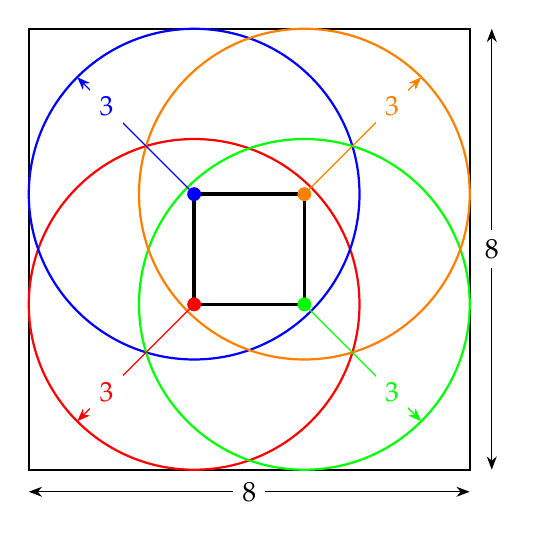
\begin{tikzpicture}[scale=.7]
\coordinate (c1) at (3,3);
\coordinate (c2) at (3,5);
\coordinate (c3) at (5,3);
\coordinate (c4) at (5,5);
\draw[very thick] (c1) -- (c3) -- (c4) -- (c2) -- cycle;
\draw[thick] (0,0) rectangle +(8,8);
\draw[color=red,thick] (c1) circle[radius=3];
\draw[color=blue,thick] (c2) circle[radius=3];
\draw[color=green,thick] (c3) circle[radius=3];
\draw[color=orange,thick] (c4) circle[radius=3];
\vertexcolor{c1}{red};
\vertexcolor{c2}{blue};
\vertexcolor{c3}{green};
\vertexcolor{c4}{orange};
\draw[<->] (0,-.4) -- node[fill=white] {$8$} (8,-.4);
\draw[<->] (8.4,0) -- node[fill=white] {$8$} (8.4,8);
\draw[->,red] (3,3) -- node[near end,fill=white] {$3$} +(-135:3);
\draw[->,blue] (3,5) -- node[near end,fill=white] {$3$} +(135:3);
\draw[->,green] (5,3) -- node[near end,fill=white] {$3$} +(-45:3);
\draw[->,orange] (5,5) -- node[near end,fill=white] {$3$} +(45:3);
\end{tikzpicture}
\end{center}
\caption{Boundaries for coins not intersecting a square}\label{f.coins1}
\end{figure}

\ans{2} The expectation is negative:
\[
E(\textsf{winnings per throw})=5\cdot\frac{1}{16}\,+\,(-1)\cdot\frac{15}{16}=-\frac{10}{16}=-0.625\,.
\]

\ans{3} Figure~\ref{f.coins2} shows four circles inscribed in the corners of the square. The side of the inner square is $a-2r$ so:
\[
P(\textsf{coin lands within the square})=\frac{(a-2r)^2}{a^2}\,.
\]
\begin{figure}[tb]
\begin{center}
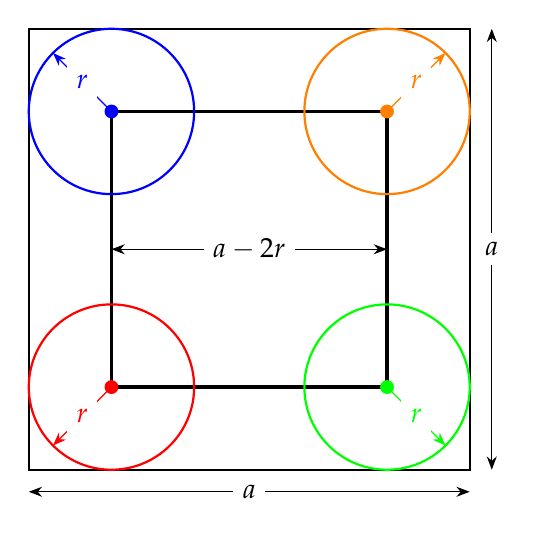
\begin{tikzpicture}[scale=.7]
\coordinate (c1) at (1.5,1.5);
\coordinate (c2) at (1.5,6.5);
\coordinate (c3) at (6.5,1.5);
\coordinate (c4) at (6.5,6.5);
\draw[very thick] (c1) -- (c3) -- (c4) -- (c2) -- cycle;
\draw[thick] (0,0) rectangle +(8,8);
\draw[color=red,thick] (c1) circle[radius=1.5];
\draw[color=blue,thick] (c2) circle[radius=1.5];
\draw[color=green,thick] (c3) circle[radius=1.5];
\draw[color=orange,thick] (c4) circle[radius=1.5];
\vertexcolor{c1}{red};
\vertexcolor{c2}{blue};
\vertexcolor{c3}{green};
\vertexcolor{c4}{orange};
\draw[<->] (0,-.4) -- node[fill=white] {$a$} (8,-.4);
\draw[<->] (8.4,0) -- node[fill=white] {$a$} (8.4,8);
\draw[->,red] (1.5,1.5) -- node[fill=white] {$r$} +(-135:1.5);
\draw[->,blue] (1.5,6.5) -- node[fill=white] {$r$} +(135:1.5);
\draw[->,green] (6.5,1.5) -- node[fill=white] {$r$} +(-45:1.5);
\draw[->,orange] (6.5,6.5) -- node[fill=white] {$r$} +(45:1.5);
\draw[<->] (1.5,4) -- node[fill=white] {$a-2r$} (6.5,4);
\end{tikzpicture}
\end{center}
\caption{Coins in a large square}\label{f.coins2}
\end{figure}

\textbf{Simulation}
\begin{verbatim}
For side = 8, radius = 1:
Probability of landing within the square = 0.5625
Proportion landing within the square     = 0.5704
For side = 8, radius = 2:
Probability of landing within the square = 0.2500
Proportion landing within the square     = 0.2481
For side = 8, radius = 3:
Probability of landing within the square = 0.0625
Proportion landing within the square     = 0.0639
For side = 8, radius = 4:
Probability of landing within the square = 0.0000
Proportion landing within the square     = 0.0000
\end{verbatim}

%%%%%%%%%%%%%%%%%%%%%%%%%%%%%%%%%%%%%%%%%%%%%%%%%%%%%%%%%%%%%

\begin{prob}{Chuck-a-luck\annotate{S}}
Choose number $n$ between $1$ and $6$. Throw three dice. If $n$ does not appear on any of the dice you lose $1$; if $n$ appears on one die you win $1$; if $n$ appears on two dice you win $2$; if $n$ appears on three dice you win $3$. What is the expectation of your winnings?
\end{prob}
\solution{}

Let $P(k)$ be the probability of $n$ appearing on $k$ dice. Then:
\[
E(\textsf{winnings per throw})=-1 P(0) + 1 P(1) + 2 P(2) + 3 P(3)\,.
\]
The throws of the three dice are independent so each of these probabilities is given by the binomial distribution with $p=1/6$, the probability that $n$ appears on a die:
\begin{eqn}
E(\textsf{winnings per throw}) &=& 
-1 \dischoose{3}{0}\left(\frac{1}{6}\right)^0\left(\frac{5}{6}\right)^3
+1\dischoose{3}{1}\left(\frac{1}{6}\right)^1\left(\frac{5}{6}\right)^2+\\
&&2{3\choose 2}\left(\frac{1}{6}\right)^2\left(\frac{5}{6}\right)^1+
3\dischoose{3}{3}\left(\frac{1}{6}\right)^3\left(\frac{5}{6}\right)^0\\
&=& \frac{1}{216}(-125+75+30+3)\\
&=&-\frac{17}{216}\approx -0.0787\,.
\end{eqn}

\textbf{Simulation}
\begin{verbatim}
Expectation of winnings = -0.0787
Average winnings        = -0.0724
\end{verbatim}

%%%%%%%%%%%%%%%%%%%%%%%%%%%%%%%%%%%%%%%%%%%%%%%%%%%%%%%%%%%%%

\begin{prob}{Curing the compulsive gambler\annotate{S}}
Roulette is a game played with a wheel having $38$ numbered pockets: $18$ red, $18$ black and $2$ green.\footnote{There are two green pockets in American roulette and one green pocket in European roulette.} The wheel is spun and a ball lands in one of the pockets. The casino wins if the ball lands in a green pocket; otherwise, you win $36$ for each $1$ bet on the number of the (red or black) pocket where the ball lands. You play $36$ rounds of roulette,  betting $1$ in each round.

\que{1} What is the expectation your winnings?

\que{2} Your friend offers to bet you $20$ that after $36$ rounds you will have \emph{lost} money. What is the expectation of your winnings, taking into account the money won or lost from both the game and your friend's bet?
\end{prob}
\solution{}

\ans{1} The probability of winning a single round is $1/38$ so:
\begin{eqn}
E(\textsf{winning one round})&=&35\cdot \frac{1}{38} + (-1)\cdot\frac{37}{38} = -\frac{2}{38} \approx -0.0526\\
E(\textsf{winning}\;36\;\textsf{rounds})&=&36\cdot -0.05266=-1.8947\,.
\end{eqn}
(Your net win is $35$ because the $36$ you receive includes your bet of $1$ which is returned.)

\ans{2}
Consider the four outcomes of playing roulette for $36$ rounds:
\begin{itemize}
\item If you lose all the rounds, you lose $36$.
\item If you win one round, you win $35$ and lose $35$ on the other rounds no money is won or lost.
\item If you win two rounds, you win $70$ and lose $34$ on the other rounds for a net win of $36$.
\item If you win $k$ rounds for $2<k\leq 36$, your net win is $35k - (36-k)>0$.
\end{itemize}
Therefore, you lose the bet only if you lose all rounds:
\[
P(\textrm{losing\ } 36 \textrm{\ rounds})=\left(\frac{37}{38}\right)^{36}\approx 0.3829\,.
\]
The probability of not losing all rounds is $1-0.3829=0.6171$. Therefore:
\[
\overbrace{-1.8947}^{\textsf{\small E of all rounds}}+\;\;
\overbrace{-20\cdot 0.3829}^{\textsf{\small lose bet}} \;+\; \overbrace{20\cdot 0.6171}^{\textsf{\small win bet}} \approx 2.7904\,.
\]
Clearly you should take the bet!

\textbf{Simulation}
\begin{verbatim}
Expectation of winning a round = -0.0526
Average winnings for a round   = -0.0593
\end{verbatim}
The simulation showed a large variance which was reduced by running one million trials.

%%%%%%%%%%%%%%%%%%%%%%%%%%%%%%%%%%%%%%%%%%%%%%%%%%%%%%%%%%%%%

\begin{prob}{Perfect bridge hand}
Randomly select $13$ cards from a deck. What is the probability that they will all be of the same suit?
\end{prob}
\solution{1}

Since there are $13$ cards of each suit there are $\dischoose{52}{13}$ ways of selecting $13$ cards of a single suit, say hearts. Only one of them consists of $13$ hearts so:
\[
P(\textsf{selecting}\;13\;\textsf{hearts})=\frac{1}{\dischoose{52}{13}}=\frac{13! 39!}{52!}=\approx 1.5747\times 10^{-12}\,.
\]
There are four suits so:
\[
P(\textsf{selecting}\;13\;\textsf{cards of the same suit})=4\cdot \frac{13! 39!}{52!}\approx 6.2991\times 10^{-12}\,.
\]

\solution{2}

There are $52$ ways of selecting the first card. Then there are $12$ ways of selecting the second card of the same suit from the remaining $51$ cards, $11$ ways of selecting a third card, and so on. Therefore:
\[
P(\textsf{selecting}\;13\;\textsf{cards of the same suit})=\frac{52}{52}\cdot \frac{12}{51}\cdot \frac{11}{50} \cdots  \frac{1}{40}= \frac{12!}{51!/39!}\approx 6.2991\times 10^{-12}\,.
\]
There is no point in running a simulation because the result would almost certainly be zero.

%%%%%%%%%%%%%%%%%%%%%%%%%%%%%%%%%%%%%%%%%%%%%%%%%%%%%%%%%%%%%

\begin{prob}{Craps\annotate{D,S}}
Craps is a played with a pair of dice. On the first throw you win if the sum of the numbers is $7$ or $11$ and you lose if the sum is $2$, $3$ or $12$. If the sum on the first throw is $n=4,5,6,8,9,10$ (called a \emph{point}), continue to throw the dice until the sum is the point $n$ (a win) or $7$ (a loss).

\que{1} What are the probabilities of the events on the first throw: winning, losing, neither?

\que{2} What is the probability of a win?
\end{prob}
\solution{1}

\ans{1} The probability of any outcome in a throw of a die is uniformly distributed and is equal to $1/6$. Since the outcomes of a throw of a pair of dice are independent, the probability of any outcome is $1/36$. The number of ways of obtaining each of the events (the sums of a pair of dice) $2,\ldots,12$ is:
\[
\begin{array}{l|rrrrrrrrrrr}
\textrm{Sum} & 2 & 3 & 4 & 5 & 6 & 7 & 8 & 9 & 10 & 11 & 12\\\hline
\textrm{Pairs} & 1 & 2 & 3 & 4 & 5 & 6 & 5 & 4 & 3 & 2 & 1
\end{array}
\]
On the first throw there are $8$ ways of throwing $7$ or $11$ for a probability of $8/36$ for winning, and $4$ ways of throwing $2,3,12$ for a probability of $4/36$ for losing. The probability of neither winning nor losing on the first throw is:
\[
1 - \frac{8}{36} - \frac{4}{36} = \frac{24}{36}\,.
\]

\ans{2}
Consider two cases referring to the table above:
\begin{itemize}
\item The point is $4$. The probability of winning on the second throw (a $4$) is $3/36$ and the probability of losing (a $7$) is $6/36$. The probability of neither winning nor losing is $1-(3/36)-(6/36)=27/36$.
\item The point is $8$. The probability of winning on the second throw (an $8$) is $5/36$ and the probability of losing (a $7$) is $6/36$. The probability of neither winning nor losing is $1-(5/36)-(6/36)=25/36$.
\end{itemize}
We see that the probability of winning must be computed separately for each of the points $4,5,6,8,9,10$. We develop a general formula for the probability.

After throwing a \emph{point} of the first throw, let $P_n$ be the probability of winning by throwing the point $n$ on a thrown and let $Q_n$ the probability of neither winning nor losing on a throw. $W_n$, the probability of winning by \emph{eventually} throwing the point $n$ after the first throw, is computed by adding:
\begin{itemize}
\item The probability of throwing the point on the second throw.
\item The probability of neither winning nor losing on the second throw and throwing the point on the third throw.
\item The probability of neither winning nor losing on the second and third throws and throwing the point on the fourth throw,
\end{itemize}
and so on.
\begin{eqn}
W_n&=&P_n + Q_n P_n + Q_n^2 P_n+ Q_n^3 P_n  + \cdots\\
&=&P_n\left(1+Q_n^1 + Q_n^2+ Q_n^3  + \cdots\right)\\
&=&P_n\left(\frac{1}{1-Q_n}\right)\,.
\end{eqn}
You lose the game on any throw after the first if you throw a $7$ with probability $6/36$ so:
\begin{eqn}
Q_n &=& 1-P_n-(6/36)\\
W_n&=&\frac{P_n}{P_n+(6/36)}\,.
\end{eqn}
$W_n$ for the six points are:
\[
\renewcommand{\arraystretch}{2}
\begin{array}{lcccccc}
n   & 4 & 5 & 6 & 8 & 9 & 10 \\\hline
P_n & \disfrac{3}{36} & \disfrac{4}{36} & \disfrac{5}{36} & \disfrac{5}{36} & \disfrac{4}{36} & \disfrac{3}{36} \\
%1-Q_n & \disfrac{9}{36} & \disfrac{10}{36} & \disfrac{11}{36} & \disfrac{11}{36} & \disfrac{10}{36} & \disfrac{9}{36} \\
W_n & \disfrac{3}{9} & \disfrac{4}{10} & \disfrac{5}{11} & \disfrac{5}{11} & \disfrac{4}{10} & \disfrac{3}{9}
\end{array}
\]
$W$, the probability of winning, can be computed by adding the probability of winning on the first throw to the sum of the probabilities for the six wins on points each multiplied by the probability of throwing \emph{that point} on the first throw:
\begin{equation}\label{eq.9-a}
W=\frac{8}{36}+\sum_{n\in\{4,5,6,8,9,10\}} P_nW_n \approx 0.4929\,.
\end{equation}
The casino's probability of winning a single game of craps is
only $0.5-0.4949\approx 0.5\%$ but the law of large numbers ensures that they will eventually win and you will eventually lose!

\solution{2}

\ans{2} Consider the following sequences of throws where in all sequences the point is $4$:
\[
\begin{array}{rrrrrrrrrrr}
4 & 8 & 9 & 9 & 9 & 8 & 8 & 8 & 9 & 8 & 4\\
4 & 8 & 9 & 9 & 9 & 8 & 8 & 8 & 9 & 8 & 7\\
4 & 9 & 9 & 9 & 8 & 8 & 4
\end{array}
\]
The games only terminates if a $4$ is thrown (win) or a $7$ is thrown (loss), so an appearance of an $8$ or a $9$ doesn't affect the result! Therefore, once a point has been thrown, the probability of winning is the conditional probability that a $4$ is thrown given that a $4$ or  a $7$ is thrown. Let $f$ be the event that a $4$ is thrown and $s$ be the event that a $7$ is thrown. Then:
\[
P(f|f\cup s) = \disfrac{P(f)\cap P(f\cup s)}{P(f\cup s)}=\disfrac{P(f)}{P(f\cup s)}=\disfrac{3/36}{(3+6)/36}=\disfrac{3}{9}\,,
\]
exactly the result $W_4$ in the table above. Equation~\ref{eq.9-a} can now be used to compute $W$.

Conditional probability is implicitly used in the first solution because $W_n$ is a probability that is conditional on the first throw resulting in the point $n$.

\textbf{Simulation}
\begin{verbatim}
Probability of winning = 0.4929
Proportion of wins     = 0.4948
\end{verbatim}

%%%%%%%%%%%%%%%%%%%%%%%%%%%%%%%%%%%%%%%%%%%%%%%%%%%%%%%%%%%%%

\refstepcounter{problem}  % 10. An experiment in personal taste


% !TeX root = mos-he.tex

%%%%%%%%%%%%%%%%%%%%%%%%%%%%%%%%%%%%%%%%%%%%%%%%%%%%%%%%%%%%%%%%

\begin{prob}{לדגום עם או בלי החזרות?}{D}{(Should you sample with or without replacement?)}

בכד 
$A$
נמצאים
$2$
כדורים אדומים וכדור ירוק אחד, ובכד 
$B$
נמצאים
$101$
כדורים אדומים ו-%
$100$
כדורים ירוקים. בחר כד אחד בצורה אקראי ושלוף שני כדורים באופן אקראי מהכד שנבחר. אתה מנצח אם אתה מזהה נכון אם כדורים נשלפו מכד 
$A$
או כד
$B$.

חשב את ההסתברויות לניצחון בכל אחד מהחוקים שלהן וקבע איזו שיטה נותן את ההסתברות הגבוהה ביותר לניצחון.

\que{1}
אתה מחזיר את הכדור הראשון לפני השליפה השנייה.

\que{2} 
אתה לא מחזיר את הכדור הראשון לפני השליפה השנייה.

\que{3}
לאחר שליפת הכדור הראשון אתה יכול להחליט אם להחזיר אותו או לא.

\textbf{רמז:} 
כאשר מחשבים הסתברויות:
\[
\disfrac{101}{201}\approx \disfrac{100}{201} \approx \disfrac{100}{200} \approx \disfrac{1}{2}\,.
\]
\end{prob}
\vspace{-6ex}

\solution{}

יש ארבע תוצאות שנסמן
$RR, RG, GR, GG$.
לכל אחד מהחוקים נחשב את ההסתברויות המתנות של ארבעת התוצאות כתלות בזהות הכד 
$A$
או
$B$
שנבחר תחילה. אחר כך נכפיל את ההסתברויות ב-%
$1/2$
כדי לקחת בחשבון את הבחירה האקראית של הכד.

\ans{1}
שליפה עם החזרה:
\[
\renewcommand*{\arraystretch}{1.5}
\begin{array}{lcccc}
P(RR|A) &=& \frac{2}{3} \cdot \frac{2}{3} &=& \frac{4}{9}\\
P(RR|B) &=& \frac{1}{2} \cdot \frac{1}{2} &=& \frac{1}{4}\\
\hline
P(RG|A) &=& \frac{2}{3} \cdot \frac{1}{3} &=& \frac{2}{9}\\
P(RG|B) &=& \frac{1}{2} \cdot \frac{1}{2} &=& \frac{1}{4}\\
\hline
P(GR|A) &=& \frac{1}{3} \cdot \frac{2}{3} &=& \frac{2}{9}\\
P(GR|B) &=& \frac{1}{2} \cdot \frac{1}{2} &=& \frac{1}{4}\\
\hline
P(GG|A) &=& \frac{1}{3} \cdot \frac{1}{3} &=& \frac{1}{9}\\
P(GG|B) &=& \frac{1}{2} \cdot \frac{1}{2} &=& \frac{1}{4}\end{array}
\]
אם התוצאה היא
$RR$
ההסתברות שכד 
$A$
נבחר
($4/9$)
גבוהה מהסתברות שכד
$B$
נבחר
($1/4$);
אחרת, ההסתברות ש-%
$B$
נבחר גבוהה יותר. לכן:
\[
P(\textrm{ניצחון})=\frac{1}{2}\left(\frac{4}{9} + \frac{1}{4}+ \frac{1}{4}+ \frac{1}{4}\right)=\disfrac{43}{72}\approx 0.5972\,.
\]

\ans{2}
שליפה ללא החזרה:
\[
\renewcommand*{\arraystretch}{1.5}
\begin{array}{lcccc}
P(RR|A) &=& \frac{2}{3} \cdot \frac{1}{2} &=& \frac{1}{3}\\
P(RR|B) &=& \frac{1}{2} \cdot \frac{1}{2} &=& \frac{1}{4}\\
\hline
P(RG|A) &=& \frac{2}{3} \cdot \frac{1}{2} &=& \frac{1}{3}\\
P(RG|B) &=& \frac{1}{2} \cdot \frac{1}{2} &=& \frac{1}{4}\\
\hline
P(GR|A) &=& \frac{1}{3} \cdot 1 &=& \frac{1}{3}\\
P(GR|B) &=& \frac{1}{2} \cdot \frac{1}{2} &=& \frac{1}{4}\\
\hline
P(GG|A) &=& \frac{1}{3} \cdot 0 &=& 0\\
P(GG|B) &=& \frac{1}{2} \cdot \frac{1}{2} &=& \frac{1}{4}
\end{array}
\]
אם התוצאה היא
$GG$
ההסתברות שכד
$B$
נבחר גבוהה יותר (כמובן!) מההסתברות שכד
$A$
נבחר; אחרת, ההסתברות שכד 
$A$
נבחר גבוהה יותר. לכן:
\[
P(\textrm{ניצחון})=\frac{1}{2}\left(\frac{1}{3} + \frac{1}{3}+ \frac{1}{3}+ \frac{1}{4}\right)=\frac{5}{8}=0.6250\,,
\]
שהיא גבוהה יותר מההסתברות לניצחון כאשר שליפה היא עם החזרה.

\ans{3} 
ההחלטה נעשית על סמך התוצאות של השליפה הראשונה.

אם השליפה הראשונה היא מכד
$A$
ההסתברויות חייבות להיות מותנות גם בהחלטה להחזיר או לא. אם השליפה הראשונה היא מכד
$B$
היא לא משפיעה על ההסתברויות בגלל הקירוב ברמז.
\[
\renewcommand*{\arraystretch}{1.5}
\begin{array}{lcccc}
P(RR|A,w) &=& \frac{2}{3} \cdot \frac{2}{3} &=& \frac{4}{9}\\
P(RR|A,w/o) &=& \frac{2}{3} \cdot \frac{1}{2} &=& \frac{1}{3}\\
P(RR|B) &=& \frac{1}{2} \cdot \frac{1}{2} &=& \frac{1}{4}\\
\hline
P(RG|A,w) &=& \frac{2}{3} \cdot \frac{1}{3} &=& \frac{2}{9}\\
P(RG|A,w/o) &=& \frac{2}{3} \cdot \frac{1}{2} &=& \frac{1}{3}\\
P(RG|B) &=& \frac{1}{2} \cdot \frac{1}{2} &=& \frac{1}{4}\\
\hline
\end{array}
\]
\[
\renewcommand*{\arraystretch}{1.5}
\begin{array}{lcccc}
P(GR|A,w) &=& \frac{1}{3} \cdot \frac{2}{3} &=& \frac{2}{9}\\
P(GR|A,w/o) &=& \frac{1}{3} \cdot 1 &=& \frac{1}{3}\\
P(GR|B) &=& \frac{1}{2} \cdot \frac{1}{2} &=& \frac{1}{4}\\
\hline
P(GG|A,w) &=& \frac{1}{3} \cdot \frac{1}{3} &=& \frac{1}{9}\\
P(GG|A,w/o) &=& \frac{1}{3} \cdot 0 &=&0\\
P(GG|B) &=& \frac{1}{2} \cdot \frac{1}{2} &=& \frac{1}{4}\\\end{array}
\]
אם כדור אדום נשלף ראשונה אזי 
$\frac{4}{9}>\frac{1}{4}$
ו-%
$\frac{2}{9}<\frac{1}{4}$
עם החזרה, לעומת
$\frac{1}{3}>\frac{1}{4}$
ו-%
$\frac{1}{3}>\frac{1}{4}$
ללא החזרה, לכן הכדור השני יכול לעזור בזיהוי הכד רק אם השליפה נעשית 
\textbf{עם}
החזרה: אם אדום כד
$A$
ואם ירוק כד
$B$.
נבחר שליפה עם החזרה:
\[
P(\textrm{ראשון אדום אם ניצחון})=\frac{1}{2}\left(\frac{4}{9}+\frac{1}{4}\right)=\frac{25}{72}\,.
\]
אם כדור ירוק נשלף ראשון אזי
$\frac{2}{9}<\frac{1}{4}$
ו-%
$\frac{1}{9}<\frac{1}{4}$
עם החזרה, לעומת
$\frac{1}{3}>\frac{1}{4}$
ו-%
$0<\frac{1}{4}$
ללא החזרה, לכן הכדור השני יכול לעזור בזיהוי הכד רק אם השליפה נעשית 
\textbf{בלי}
החזרה:
\[
P(\textrm{ראשון ירוק אם ניצחון})=\frac{1}{2}\left(\frac{1}{3}+\frac{1}{4}\right)=\frac{7}{24}\,.
\]
ההסתברות לניצחון היא:
\[
P(\textrm{ניצחון})=\frac{25}{72} + \frac{7}{24}=\frac{23}{36}\approx 0.6389\,.
\]
ההסתברות הגבוהה ביותר לניצחון מתקבלת כאשר ההחלטה לשלוף עם או בלי החזרה מתקבלת בהתאם לתוצאה של השליפה הראשונה.

\sml{}

\selectlanguage{english}
\begin{verbatim}
With replacement:
Expectation of winning = 0.5972
Average wins           = 0.5976
Without replacement:
Expectation of winning = 0.6250
Average wins           = 0.6207
Decide after first draw:
Expectation of winning = 0.6389
Average wins           = 0.6379
\end{verbatim}
\selectlanguage{hebrew}

%%%%%%%%%%%%%%%%%%%%%%%%%%%%%%%%%%%%%%%%%%%%%%%%%%%%%%%%%%%%%

\newpage

\begin{prob}{הקלפי}{}{(The ballot box)}

שני מועמדים
$A$
ו-%
$B$
מתמודדים בבחירות. 
$A$
קיבל
$a$
קולות ו-%
$B$
קיבל
$b$
קולות,
$a>b$.
הקולות נספרים אחד-אחד וסכומי הביניים
$(a_i,b_i), 1\leq i \leq a+b$
מתעדכנים לאחר ספירת כל קול. מה ההסתברות שעבור לפחות
$i$
אחד,
$a_i=b_i$?

\que{1} 
פתור עבור
$a=3, b=2$
על ידי הכנת רשימה
$(a_i,b_i)$
עבור
$1\leq i\leq 5$.

\que{2} 
פתור לכל
$a>b$.

\textbf{רמז 1:} 
מה ניתן להגיד על זהות המועמד המוביל עד לתיקו 
\textbf{הראשון}?

\textbf{רמז 2:}
מה החשיבות של הקול הראשון שנספר.
\end{prob}

\solution{}

\ans{1}
מספר הדרכים לסדר את סכומי הביניים הוא
${5\choose 2}={5\choose 3}=10$ 
כי המיקום הקולות עבור מועמד אחד קובע את מיקום הקולות של המועמד השני. בטבלה שלהלן רשומים הסידורים האפשריים של הקולות וסכומי הביניים כאשר התיקו הראשון מודגש:
\begin{center}
\begin{minipage}{.48\textwidth}
\[
\begin{array}{ccccc}
A & A & A & B & B\\
A & A & B & A & B\\
A & B & A & A & B\\
B & A & A & A & B\\%\hline
A & A & B & B & A\\
A & B & A & B & A\\
B & A & A & B & A\\%\hline
A & B & B & A & A\\
B & A & B & A & A\\%\hline
B & B & A & A & A
\end{array}
\]
\end{minipage}
\hspace{-4em}
\begin{minipage}{.48\textwidth}
\[
\begin{array}{rrrrr}
%(4,5)&
(1,0) & (2,0) & (3,0) & (3,1) & (3,2)\\
%(3,5)&
(1,0) & (2,0) & (2,1) & (3,1) & (3,2)\\
%(2,5)&
(1,0) & \mathbf{(1,1)} & (2,1) & (3,1) & (3,2)\\
%(1,5)&
(0,1) & \mathbf{(1,1)} & (2,1) & (3,1) & (3,2)\\%\hline
%(3,4)&
(1,0) & (2,0) & (2,1) & \mathbf{(2,2)} & (3,2)\\
%(2,4)&
(1,0) & \mathbf{(1,1)} & (2,1) & (2,2) & (3,2)\\
%(1,4)&
(0,1) & \mathbf{(1,1)} & (2,1) & (2,2) & (3,2)\\%\hline
%(2,3)&
(1,0) & \mathbf{(1,1)} & (1,2) & (2,2) & (3,2)\\
%(1,3)&
(0,1) & \mathbf{(1,1)} & (1,2) & (2,2) & (3,2)\\%\hline
%(1,2)&
(0,1) & (0,2) & (1,2) &  \mathbf{(2,2)} & (3,2)
\end{array}
\]
\end{minipage}
\end{center}
קיימים מצבי תיקו בכל הסידורים פרט לשני הראשונים ולכן:
\[
P(\textrm{קולות}\;(3,2)\;\textrm{עם תיקו קיים})=\disfrac{8}{10}=\disfrac{4}{5}\,.
\]

\ans{2} 
נתחיל עם דיון איך לגשת לפתרון של השאלה השנייה. הנה מספר סידורים עבור 
$(a,b)=(3,2)$
עד לקבלת
\textbf{התיקו הראשון}:
\[
\begin{array}{rrrrr|rrrrr}
\multicolumn{5}{c|}{\textrm{תיקו עד מוביל}\;A} &
\multicolumn{5}{c}{\textrm{תיקו עד מוביל}\;B}\\\hline
A & B &&& &B & A & & &\\
A & A & B & B && B & B & A & A&\\
\end{array}
\]
לכל סידור בו 
$A$
מוביל עד לתיקו הראשון, קיים סידור שהוא תמונת ראי בו 
$B$
מוביל עד לקבלת התיקו הראשון. השיקוף מתקבל על ידי החלפת כל 
$A$
ב-%
$B$
ולהפך. לפני התיקו הראשון אחד מהמועמדים חייב להוביל. אם הקול הראשון שנספר הוא עבור 
$B$
חייב להיות תיקו בהמשך הספירה כי
$a>b$.

ההסתברות שהקול הראשון היא עבור 
$B$
היא:
\[
P(B\;\textrm{עבור ראשון קול})=\frac{b}{a+b}\,.
\]
על ידי שיקוף המיקומים של הקולות, מספר הסידורים שמובילים לתיקו שמתחילים בקול עבור
$A$
שווה למספר הסידורים שמובילים לתיקו שמתחילים בקול עבור
$B$. 
לכן:
\[
P(\textrm{תיקו קיים })=2\cdot\frac{b}{a+b}\,.
\]
בדיקה:
\[
P(\textrm{קולות}\;(3,2)\;\textrm{עם תיקו קיים})=2\cdot\frac{2}{2+3}=\frac{4}{5}\,.
\]

\sml{}

\selectlanguage{english}
\begin{verbatim}
For a =  3, b =  2:
Probability of a tie = 0.8000
Proportion of ties   = 0.8118
For a = 10, b =  8:
Probability of a tie = 0.8889
Proportion of ties   = 0.8977
For a = 20, b = 18:
Probability of a tie = 0.9474
Proportion of ties   = 0.9354
\end{verbatim}
\selectlanguage{hebrew}


%%%%%%%%%%%%%%%%%%%%%%%%%%%%%%%%%%%%%%%%%%%%%%%%%%%%%%%%%%%%%

\begin{prob}{תיקו בהשוואת מטבעות}{D}{(Ties in matching pennies)}

הטל זוג מטבעות הוגנות
$N$
פעמים עבור
$N$
זוג, ורשום את מספר הפעמים שהזוגיות היא זוגי (עץ-עץ או פלי-פלי) ומספר ההפעמים שהזוגיות היא אי-זוגי (עץ-פלי או פלי-עץ). מה ההסתברות לקבל תיקו (לא כולל התיקו 
$0-0$
בהתחלה)?

\que{1}
פתור עבור 
$N=4$
על ידי רישום כל התוצאות האפשריות.

\que{2} 
פתור עבור
$N=6$
על ידי פיתוח נוסחה להסתברות.

\que{3}
הסבר מדוע ההסתברות למספר אי-זוגי
$N+1$
שווה להסתברות של המספר הזוגי
$N$.

\textbf{רמז:}
השתמש בפתרון לבעיה%
~$22$.
\end{prob}

\solution{}

\ans{1} 
נסמן את ההטלות עם זוגיות זוגי ב-%
$E$
וההטלות עם זוגיות אי-זוגי ב-%
$O$.
בעשרה מתוך ששה עשר סידורי ההטלות יש תיקו (מודגש):
\begin{center}
\begin{tabular}{llllllll}
EEEE & EEEO & EEOE & \textbf{EEOO} & \textbf{EOEE} & \textbf{EOEO} &\textbf{EOOE} & \textbf{EOOO}\\
\textbf{OEEE} & \textbf{OEEO} & \textbf{OEOE} & \textbf{OEOO} & \textbf{OOEE} & OOEO&OOOE & OOOO
\end{tabular}
\end{center}

\ans{2}
לפי בעיה~22:
\begin{equation}\label{eq.coins-ties}
P(i\;\textrm{בהטלה תיקו})=
\left\{
\begin{array}{ll}
2i/N & i\leq N/2\;\textrm{אם}\\
2(N-i)/N&i\geq N/2\;\textrm{אם}\,,
\end{array}
\right.
\end{equation}
כי בבעיית הקלפי הראנו שהערך הנמוך יותר קובע את ההסתברות.

ההסתברות ל-%
$i$
זוגיים ניתן על ידי ההתפלגות הבינומית:
\begin{equation}\label{eq.coins00}
P(i\;\textrm{זוגיים})=\dischoose{N}{i} \left(\disfrac{1}{2}\right)^i \left(\disfrac{1}{2}\right)^{N-i}=\dischoose{N}{i} \left(\disfrac{1}{2}\right)^N =  2^{-N}\dischoose{N}{i}\,.
\end{equation}
ההסתברות לתיקו היא הסכום מעל 
$i$
של ההסתברות לקבל 
$i$
זוגיים כפול ההסתברות לתיקו בהטלה ה-%
$i$
(משוואה%
~\ref{eq.coins-ties}).
עבור
$N=6$
ותוך שימוש ב-%
${N \choose i}={N\choose N-i}$:
\begin{eqn}
P(\textrm{תיקו})&=&\disfrac{2\cdot 2^{-6}}{6}\sum_{i=0}^{6}i\dischoose{i}{6}\\
%
&=&\disfrac{1}{192}\left(
0\cdot \dischoose{6}{0}+
1\cdot \dischoose{6}{1}+
2\cdot \dischoose{6}{2}+
3\cdot \dischoose{6}{3}+
4\cdot \dischoose{6}{2}+
5\cdot \dischoose{6}{1}+
6\cdot \dischoose{6}{0}
\right)\\
%
&=&\disfrac{1}{192}\left(
2\cdot \dischoose{6}{1}+
4\cdot \dischoose{6}{2}+
3\cdot \dischoose{6}{3}
\right)\\
&=&\disfrac{132}{192}\approx 0.6875\,.
\end{eqn}%

\ans{3}
התיקו הראשון בהטלה ה-%
$N+1$
מתרחש רק עם הספירה כמעט זהות לאחר ההטלה ה-%
$N$:
\[
\begin{array}{l}
((N/2)-1,(N/2)+1)\\((N/2),(N/2))\\((N/2)+1,(N/2)-1)
\end{array}
\]
אבל ללא תלות התוצאת ההטלה הסופית הערכים לא יהיו שווים.

\sml{}
\selectlanguage{english}
\begin{verbatim}
For  4 tosses:
Probability of ties = 0.6250
Proportion of ties  = 0.6192
For  6 tosses:
Probability of ties = 0.6875
Proportion of ties  = 0.6900
For  7 tosses:
Probability of ties = 0.6875
Proportion of ties  = 0.6811
For 10 tosses:
Probability of ties = 0.7539
Proportion of ties  = 0.7559
For 20 tosses:
Probability of ties = 0.8238
Proportion of ties  = 0.8255
\end{verbatim}
\selectlanguage{hebrew}

%%%%%%%%%%%%%%%%%%%%%%%%%%%%%%%%%%%%%%%%%%%%%%%%%%%%%%%%%%%%%

\refstepcounter{problem} % 24. The unfair subway

%%%%%%%%%%%%%%%%%%%%%%%%%%%%%%%%%%%%%%%%%%%%%%%%%%%%%%%%%%%%%



\begin{prob}{אורכים של מיתרים אקראיים}{}{(Lengths of random chords)}

בחר מיתר אקראי במעגל היחידה. מה ההסתברות שאורכו של המיתר גדול מ-%
$1$?

כדי לפתור את הבעיה עליך להחליט איך לבחור מיתר אקראי. פתור את הבעיה עבור מהאפשרויות שלהלן:

\que{1} 
התפלגות אחידה של מרחק המיתר מהמרכז המעגל.

\que{2}
התפלגות אחידה של הנקודה האמצעית של המיתר בתוך המעגל.

\que{3}
התפלגות נקודות הקצה של המיתר על היקף המעגל.
\end{prob}

\solution{}

\ans{1}
מיתר ארוך יותר מהרדיוס אם הוא קרוב יותר למרכז ממיתר באורך 
$1$.
יהי 
$\overline{AB}$
מיתר באורך 
$1$
ובנה גובה
$h=\overline{OH}$
מהמרכז 
$O$
אל המיתר (%
\ref{f.chord1}). 
בגלל ש-%
$\triangle AOB$
שווה-צלעות
$\triangle OHB$ 
הוא משולש ישר-זווית:
\[
h = \sin \frac{\pi}{3} = \frac{\sqrt{3}}{2}\,.
\]
יהי
$d$
המרחק של המיתר 
$\overline{DE}$
מהמרכז. לפי ההנחה ההתפלגות של
$d$
אחידה ב-%
$(0,1)$
ולכן:
\[
P(\overline{DE}>1)=P(d<h)=\disfrac{h}{1}=\frac{\sqrt{3}}{2} \approx 0.8660\,.
\]

\begin{figure}[tb]
\centering
\selectlanguage{hebrew}
\subcaptionbox{%
מרחק של מיתר מהמרכז בהתפלגות אחידה ב-%
$(0,1)$%
\label{f.chord1}}
[.45\textwidth]
{
\centering
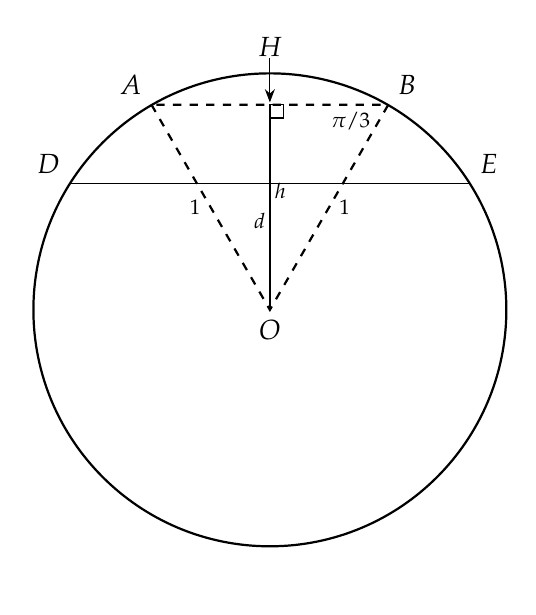
\begin{tikzpicture}[scale=.8]
\coordinate (O) at (0,0) node[below] {$O$};
\node (hexagon) [minimum size=6cm,regular polygon,
                 regular polygon sides=6] at (O) {};
\node[name path=circle,draw,thick,circle through=(hexagon.corner 1)] at (O) {};
\draw[thick,dashed] (hexagon.corner 2) -- 
  node[left] {$\scriptstyle 1$} (O) --
  node[right] {$\scriptstyle 1$} (hexagon.corner 1) -- cycle;
\node[above left] at (hexagon.corner 2) {$A$};
\node[above right] at (hexagon.corner 1) {$B$};
\coordinate (H) at (O |- hexagon.corner 1);
\node[above,yshift=14pt] at (H) {$H$};
\draw[<-] ($(H)+(0pt,1pt)$) -- +(0pt,+20pt);
\draw[thick] (O) -- 
  node[right,xshift=-2pt,yshift=6pt] {$\scriptstyle h$} 
  node[left,xshift=2pt,yshift=-5pt] {$\scriptstyle d$}
  (H);
\draw[rotate=-90] (H) rectangle +(6pt,6pt);
\node[below left,xshift=-3pt,yshift=1pt] at 
  (hexagon.corner 1) {$\scriptstyle \pi/3$};
\path (hexagon.corner 2) -- 
  (H) -- (hexagon.corner 1);
\node[xshift=15mm,yshift=-8mm]  at (hexagon.corner 4)
  {};
\path[name path=chord] (-3.5,2) -- +(7,0);
\path [name intersections={of=circle and chord,by={E,D}}];
\draw (D) node[above left] {$D$} -- (E) node[above right] {$E$};
\end{tikzpicture}
}
\hspace{3em}
\subcaptionbox{%
נקודת האמצע של מיתר בהתפלגות אחידה במעגל ונקודות הקצה של המיתר בהתפלגות אחידה בהיקף%
\label{f.chord2}}
[.45\textwidth]
{
\centering
\begin{tikzpicture}[scale=.8]
\coordinate (O) at (0,0) node[right] {$O$};
\node (hexagon) [minimum size=6cm,regular polygon,
                 regular polygon sides=6] at (O) {};
\node[draw,thick,name path=circle,
      circle through=(hexagon.corner 1)] at (O) {};
\draw[thick,dashed] (hexagon.corner 3) -- 
  node[above] {$\scriptstyle 1$} (O) --
  node[right] {$\scriptstyle 1$} (hexagon.corner 4) -- cycle;
\coordinate (H) at ($(hexagon.corner 3)!.5!(hexagon.corner 4)$);
\node[left,yshift=-25pt] at (H) {$H$};
\draw[<-] ($(H)+(-1pt,-1pt)$) -- +(-8pt,-23pt);
\draw[thick] (O) -- 
  node[above,near end] {$\scriptstyle h$} (H);
\draw[rotate=-60] (H) rectangle +(6pt,6pt);
\node[draw,thick,dashed,circle through=(H)] at (O) {};
\node[left]        at (hexagon.corner 3) {$F$};
\node[below left]  at (hexagon.corner 4) {$E$};
\node[xshift=-14mm,yshift=10mm]  at (hexagon.corner 4)
  {$\frac{\pi}{3}$};
\node[xshift=15mm,yshift=-8mm]  at (hexagon.corner 4)
  {$\frac{\pi}{3}$};
\node[below right] at (hexagon.corner 5) {$D$};
\draw[thick]  (hexagon.corner 3) -- (hexagon.corner 4) --
     node[below,yshift=1pt] {$\scriptstyle 1$}
     (hexagon.corner 5);
\node[draw,thick,name path=circle,
      circle through=(hexagon.corner 1)] at (O) {};
\path[name path=chord] (hexagon.corner 4) -- +(15:5);
\path [name intersections={of=circle and chord,by={K,L}}];
\node[left] at (L) {$G$};
\draw[ultra thick,dotted] (hexagon.corner 4) -- (L);
\coordinate (center) at ($(hexagon.corner 4)!.5!(L)$);
\fill (center) circle (2pt);
\end{tikzpicture}
}
\end{figure}

\ans{2}
בנה מעגל עם מרכז
$O$
ורדיוס 
$h$
כאשר 
$h$
הוא אורכו של גובה לגובה למיתר באורך 
$1$.
משיק לכל נקודה על המעגל יהיה מיתר
$\overline{FE}$
שאורכו 
$1$.
אורכו של כל מיתר
$\overline{EG}$
שנקודת האמצע שלו נמצאת בתוך המעגל יהיה גדול מ-%
$1$
(\ref{f.chord2}),
ולכן ההסתברות שאורכו של מיתר גדול מ-%
$1$
היא היחס בין השטחים של שני המעגלים:
\[
P(\overline{EG}>1)=\frac{\pi \cdot h^2}{\pi \cdot 1^2}=h^2=\frac{3}{4}\,.
\]
הסתברות זו היא הריבוע של ההסתברות שחישבנו בשאלה הקודמת.

\ans{3}
בנקודה שרירותית על ההיקף של מעגל היחידה (%
$E$
ב%
\ref{f.chord2}).
כל נקודה אחרת על ההיקף (כגון 
$G$
באיור) מגדירה מיתר שאורכו גדול מאחד אלא אם הנקודה שנבחרה נופל על הקשתות
$\widehat{EF}$
או
$\widehat{ED}$.
לכן ההסתברות היא היחס בין הקשת
$\widehat{FD}$
להיקף המעגל:
\[
P(\overline{EG}>1)=\frac{(2\pi-(2\pi/3))\cdot 1}{2\pi \cdot 1}=\frac{2}{3}\,.
\]

\newpage

\sml{}

הסימולציה היא עבור בחירת שתי נקודות על ההיקף.
\selectlanguage{english}
\begin{verbatim}
Probability of long chords = 0.6667
Proportion of long chords  = 0.6627
\end{verbatim}
\selectlanguage{hebrew}

%%%%%%%%%%%%%%%%%%%%%%%%%%%%%%%%%%%%%%%%%%%%%%%%%%%%%%%%%%%%%

\begin{prob}{הממהרים לדו-קרב}{}{(The hurried duelers)}

$A$
ו-%
$B$
מגיעים לנקודת מפגש בזמן אקראי עם התלפגות אחידה בתוך פרק זמן של שעה. אם 
$A$
מגיע קודם ו-%
$B$
לא מגיע במשך 
$5$
דקות, 
$A$
עוזב. באופן דומה אם 
$B$
מגיע קודם ו-%
$A$
לא מגיע במשך 
$5$
דקות,
$B$
עוזב. מה ההסתברות שהם יפגשו?

בפרק הזמן של שעה הזמן הוא
\textbf{רציף}
בתחום
$[0,1]$,
כלומר, אי-אפשר לספור מספר בדיד של דקות או שניות כדי לחשב הסתברויות. כן ניתן לחשב הסתברויות של פרקי זמן.

\textbf{רמז:}
צייר גרף כאשר ציר ה-%
$x$
הוא זמן הגעתו של
$A$
וציר ה-%
$y$
הוא זמן הגעתו של 
$B$.
\end{prob}

\solution{}

ללא הגבלת הכלליות הנח ש-%
$A$
מגיע קודם. אם 
$A$
מגיע ב-%
$t_A=0$
ואם 
$B$
מגיע לפני
$t_B=5/60$
הם נפגשים, אחרת הם לא נפגשים. מצב זה מוצג באיור%
~\ref{f.duel}
על ידי ריבוע קטן בראשית הצירים.
\begin{figure}[tb]
\begin{center}
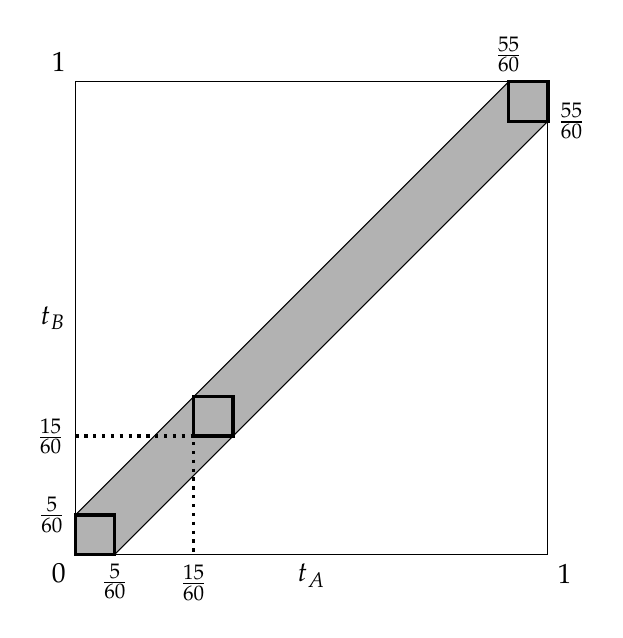
\begin{tikzpicture}
\draw (0,0) -- node[below] {$t_A$} (6,0) -- (6,6) -- (0,6) -- node[left] {$t_B$} cycle;
\node[below left]  at (0,0) {$0$};
\node[below right] at (6,0) {$1$};
\node[above left]  at (0,6) {$1$};
\draw[fill=white!70!black]
  (0,0) -- 
  (.5,0) node[below] {$\frac{5}{60}$} -- 
  (6,5.5) node[right] {$\frac{55}{60}$} --
  (6,6) -- (5.5,6) node[above] {$\frac{55}{60}$} --
  (0,.5) node[left] {$\frac{5}{60}$} -- cycle;
\draw[very thick] (0,0) -- (.5,0) -- (.5,.5) -- (0,.5) -- cycle;
\draw[very thick] (1.5,1.5) -- ++(.5,0) -- ++(0,.5) --
  ++(-.5,0) -- cycle;
\draw[very thick] (5.5,5.5) -- ++(.5,0) -- ++(0,.5) --
  ++(-.5,0) -- cycle;
\draw[very thick,dotted] (0,1.5) node[left] {$\frac{15}{60}$} --
  (1.5,1.5) -- (1.5,0) node[below] {$\frac{15}{60}$};
\end{tikzpicture}
\end{center}
\caption{זמנים המבטיחים מפגש בין $A$ ל-$B$}\label{f.duel}
\end{figure}
אם 
$A$
מגיע יותר מאוחר אזי גם
$B$
חייב להגיע באותו איחור. למשל, אם 
$A$
מגיע ב-%
$t_A=15$,
$B$
חייב להגיע בין
$t_B=15$
ו-%
$t_B=20$.
לכן הפגישה תתקיים בריבוע המתקבל על ידי הזזת הריבוע ב-%
$15$
מ-%
$(0,0)$
ל-%
$(15/60,15/60)$.

ההסתברות לפגישה היא היחס בין השטח האפור בגרף לשטחו של הריבוע הגדול. קל יותר לחשב את המשלים שהוא היחס בין שטח המשולשים הלבנים לשטחו של הריבוע הגדול:
\begin{eqn}
P(\textrm{נפגשים}\;A,B) &=& 1- P(\textrm{נפגשים לא}\;A,B)\\
&=&1- 2\cdot \left(\frac{1}{2}\cdot \frac{55}{60}\cdot \frac{55}{60}\right)=\frac{23}{144}\approx 0.1597\,.
\end{eqn}

\sml{}
\selectlanguage{english}
\begin{verbatim}
Probability of meeting   = 0.1597
Proportion of meetings   = 0.1549
\end{verbatim}
\selectlanguage{hebrew}

%%%%%%%%%%%%%%%%%%%%%%%%%%%%%%%%%%%%%%%%%%%%%%%%%%%%%%%%%%%%%

\begin{prob}{לתפוס את הזייפן הזהיר}{}{(Catching the cautious counterfeiter)}

נתון 
$n$
קופסאות ובכל אחת 
$n$
מטבעות כאשר מטבע אחד בכל קופסה מזויף. שלוף מטבע אחת מכל קופסה ובדוק אם היא מזויפת או אמיתית. מה ההסתברות שכל המטבעות שנשלפות מזויפות?

\que{1} 
פתור עבור
$n=10$.

\que{2} 
פתור עבור 
$n=100$.

\que{3}
פתח נוסחה עבור ההסתברות כאשר
$n$
שרירותי.

\que{4}
פתח נוסחה עבור ההסתברות כאשר
$n$
שואב לאיסוף.
\end{prob}

\newpage

\solution{}

השליפות בלתי תלויות ולכן ההסתברות שכל המטבעות אמיתיות היא מכפלת ההסתברות עבור שליפה אחת.

\ans{1}
\[
P(\textrm{אמיתיים המטבעות כל}) = \left(\frac{9}{10}\right)^{10}\approx 0.3487\,.
\]


\ans{2}
\[
P(\textrm{אמיתיים המטבעות כל}) = \left(\frac{99}{100}\right)^{100}\approx 0.3660\,.
\]

\ans{3}
\[
P(\textrm{אמיתיים המטבעות כל}) = \left(\frac{n-1}{n}\right)^{n}\,.
\]

\ans{4}
\begin{equation}\label{eq.reciprocal}
\lim_{n\rightarrow\infty}\left(1-\frac{1}{n}\right)^{n}=\frac{1}{e}\,.
\end{equation}

ניתן להוכיח את הגבול באמצעות חשבון דיפרנציאלי. תחילה ניתן לחשב את הגבול של הלוגריתם של הצד השמולי של משוואה%
~\ref{eq.reciprocal}:
\[
\lim_{n\rightarrow\infty}\ln \left(1-\frac{1}{n}\right)^{n}=
  \lim_{n\rightarrow\infty}n\ln \left(1-\frac{1}{n}\right)=
  \lim_{n\rightarrow\infty} \disfrac{\ln\left(1-\frac{1}{n}\right)}{1/n}\,.
\]
אם נחשב את הגבול נקבל
$(\ln \;1)/0=0/0$
אבל לפי חוק
\L{l'H\^{o}pital}
נוכל להחליף את הביטוי בחילוק הנגזרות:
\begin{eqn}
\lim_{n\rightarrow\infty}\ln \left(1-\frac{1}{n}\right)^{n}&=&\lim_{n\rightarrow\infty}\frac{\left(1-\frac{1}{n}\right)^{-1}(-(-n^{-2}))}{-n^{-2}}=-1\\
\lim_{n\rightarrow\infty}\left(1-\frac{1}{n}\right)^{n}&=&e^{-1}\approx 0.3679\,.
\end{eqn}

\sml{}
\selectlanguage{english}
\begin{verbatim}
For  10 boxes:
Probability of all real = 0.3487
Proportion all real     = 0.3480
For 100 boxes:
Probability of all real = 0.3660
Proportion all real     = 0.3730
For 200 boxes:
Probability of all real = 0.3670
Proportion all real     = 0.3690
\end{verbatim}
\selectlanguage{hebrew}

%%%%%%%%%%%%%%%%%%%%%%%%%%%%%%%%%%%%%%%%%%%%%%%%%%%%%%%%%%%%%

\begin{prob}{לתפוס את הזייפן החמדן}{}{(Catching the greedy counterfeiter)}

נתון 
$n$
קופסאות ובכל אחת 
$n$
מטבעות מהן
$m$
מזוייפות. שלוף מטבע אחת מכל קופסה ובדוק אם היא מזויפת או אמיתית. מה ההסתברות 
$P(n,m,r)$
ש-%
$r$
מתוך המטבעות מזוייפות?

\que{1} 
פתח נוסחה עבור
$P(n,m,r)$.

\que{2}
חשב
$P(20,10,2), P(20,10,8), P(20,5,2), P(20,5,4)$.
\end{prob}

\solution{}

\ans{1}
יש 
${n\choose r}$
תת-קבוצות של קבוצת הקופסאות מהן המטבעות המזוייפות נשלפו. לפי ההתפלגות הבינומית:
\[
P(n,m,r) = {n \choose r} \left(\frac{m}{n}\right)^r \left(\frac{n-m}{n}\right)^{n-r}\,.
\]

\ans{2}
\begin{eqn}
P(20,10,2) &=& \dischoose{20}{2} \left(\frac{10}{20}\right)^2 \left(\frac{10}{20}\right)^{18}\approx 0.0002\\
P(20,10,8) &=& \dischoose{20}{8} \left(\frac{10}{20}\right)^{8} \left(\frac{10}{20}\right)^{12}\approx 0.1201\\
P(20,5,2)&=&\dischoose{20}{2} \left(\frac{5}{20}\right)^2 \left(\frac{15}{20}\right)^{18}\approx 0.0669\\
P(20,5,4)&=&\dischoose{20}{4} \left(\frac{5}{20}\right)^{4} \left(\frac{15}{20}\right)^{12}\approx 0.1952\,.
\end{eqn}

\sml{}
\selectlanguage{english}
\begin{verbatim}
For 10 bad coins,  2 draws:
Probability of counterfeit  = 0.0002
Proportion counterfeit      = 0.0002
For 10 bad coins,  8 draws:
Probability of counterfeit  = 0.1201
Proportion counterfeit      = 0.1181
For  5 bad coins,  2 draws:
Probability of counterfeit  = 0.0669
Proportion counterfeit      = 0.0688
For  5 bad coins,  4 draws:
Probability of counterfeit  = 0.1897
Proportion counterfeit      = 0.1905
\end{verbatim}
\selectlanguage{hebrew}

\L{Mosteller}
משתמש בגבול מבעיה 
$27$
כדי להראות שעבור 
$m,r$
נתון, כאשר 
$n$
שואף לאינסוף:
\begin{equation}\label{eq.bin-limit}
\lim_{n\rightarrow \infty}P(n,m,r) = \frac{e^{-m}m^r}{r!}\,.
\end{equation}
הנה השוואה של ההסתברויות עבור 
$m=10, r=8$
עבור ערכים עולים של
$n$:
\selectlanguage{english}
\begin{verbatim}
Limit = 0.11259903, binomial = 0.11482303, n = 100
Limit = 0.11259903, binomial = 0.11282407, n = 1000
Limit = 0.11259903, binomial = 0.11262155, n = 10000
Limit = 0.11259903, binomial = 0.11259926, n = 1000000
\end{verbatim}
\selectlanguage{hebrew}

%%%%%%%%%%%%%%%%%%%%%%%%%%%%%%%%%%%%%%%%%%%%%%%%%%%%%%%%%%%%%

\begin{prob}{\protect עובש בג'לטין}{}{(Moldy gelatin)}

נתון לוח מלבני שמחולק ל-%
$n$
משבצות ריבועיות קטנות. בכל משבצת יש 
$r$ 
חיידקים בממוצע.

\que{1} 
פתח נוסחה להסתברות שיש בדיוק 
$r$
חיידקים ב-%
$n$
המשבצות.

\que{2}
חשב את ההסתברות עבור
$n=100,r=3$.

\textbf{רמז:}
בעיה זו דומה לבעיה%
~$28$.

\end{prob}

\solution{}

\ans{1}
$p$,
ההסתברות שבמשבצת אחת נמצא חידק (נתעלם מהאפשרות שחיידק אחד מוכל באופן חלקי בשתי משבצות או יותר), היא
$m/n$.
$P(n,m,r)$,
ההסתברות שיש בדיוק 
$r$
חיידקים ב-%
$n$
משבצות' ניתנת על ידי ההתפלגות הבינומית:
\[
P(n,m,r) = {n \choose r} \left(\frac{m}{n}\right)^r \left(\frac{n-m}{n}\right)^{n-r}\,.
\]

\ans{2} 
\[
P(10,3,3) = {100 \choose 3} \left(\frac{3}{100}\right)^3 \left(\frac{97}{100}\right)^{97}\approx 0.2275\,.
\]

\sml{}
\selectlanguage{english}
\begin{verbatim}
For  20 squares:
Probability of exactly  3 microbes  = 0.2428
Proportion of exactly   3 microbes  = 0.2436
Probability of exactly  5 microbes  = 0.2023
Proportion of exactly   5 microbes  = 0.1954
For 100 squares:
Probability of exactly  3 microbes  = 0.2275
Proportion of exactly   3 microbes  = 0.2247
Probability of exactly  5 microbes  = 0.1800
Proportion of exactly   5 microbes  = 0.1851
\end{verbatim}
\selectlanguage{hebrew}


משוואה%
~\ref{eq.bin-limit}
מתאים גם כאן לחשב את הגבול כאשר 
$n$
שואף לאינסוף:
\begin{eqnarray*}
\lim_{n\rightarrow \infty}P(n,m,r) &=& \frac{e^{-m}m^r}{r!}\\
\lim_{n\rightarrow \infty} P(n,3,3) &=& \frac{e^{-3}\cdot 3^3}{3!}\approx 0.2240\\
\lim_{n\rightarrow \infty} P(n,5,5) &=& \frac{e^{-5}\cdot 5^5}{5!}\approx 0.1755\,.
\end{eqnarray*}

%%%%%%%%%%%%%%%%%%%%%%%%%%%%%%%%%%%%%%%%%%%%%%%%%%%%%%%%%%%%%

\refstepcounter{problem} % 30. Evening the sales

%%%%%%%%%%%%%%%%%%%%%%%%%%%%%%%%%%%%%%%%%%%%%%%%%%%%%%%%%%%%%

\begin{prob}{ימי הולדת זהים}{}{(Birthday pairings)}

\que{1}
עבור 
$n$
אנשים מה ההסתברות 
$P(n)$
שלניים מהם או יותר יש יום הולדת זהה?

\que{2}
מה מערך הקטן ביותר עבור 
$n$
כך ש-%
$P(n)>0.5$?

הנח שההתפלגות של ימי ההודלת היא אחידה בטווח
$[1,365]$.

\textbf{רמז:}
חשב את המשלים להסתברות של-%
$n$
אנשים ימי הולדת 
\textbf{שונים}.
\end{prob}

\solution{}

\ans{1}
בחר 
$n$
אנשים אחד אחרי השני ובדוק אם יש להם אותו יום הולדת כמו הקודמים שנבחרו. עבור הראשון יש 
$365$
ימים, עבור השני
$364$
ימים וכך הלאה:
\[
1-P(n)=
  \overbrace{\disfrac{365}{365}\cdot\frac{364}{365}
  \cdot \;\cdots \; \cdot \frac{365-(n-2)}{365}
  \cdot\frac{365-(n-1)}{365}}^{n}
=\disfrac{365!/(365-n)!}{365^{n}}\,.
\]

\ans{2}
חשב ערך זה עבור ערכים שונים של
$n$
או השתמש בתכנית מחשב כדי לחפש מ-%
$1$
ל-%
$365$
כדי למצוא את הערך הראשון עבורו
$1-P(n)<0.5$.
הערך הוא
$23$:
\[
1-P(23)=\disfrac{365!}{365^{23}\cdot 342!}\approx 0.4927\,.
\]
רוב האנשים מופתעים שהתשובה היא ערך כל קטן.

מחשבון מודרני מסוגל לחשב 
$1-P(n)$
אבל שווה לחשב אותו באמצעות הקירוב של 
\L{Stirling}
שהוא
$\ln n! \approx n\ln n - n$:
\begin{eqnarray*}
\ln (1-P(n))&=&
  \ln\left(\disfrac{365!}{342!\cdot 365^{23}}\right)=\ln 365! - \ln 342! -23 \ln 365\\
&\approx& (365\ln 365 -365) - (342\ln 342 -342) - 23\,\ln 365 \\
&\approx&-0.7404\\
1-P(n)&\approx&e^{-0.7404}=0.4769\,.
\end{eqnarray*}
הקורא מוזמן לחשב את ההסתברות עם הקירוב המדוייק יותר:
\[
\ln n!  \approx n\ln n - n + \frac{1}{6}\left(8n^3+4n^2+n+\frac{1}{30}\right)+\frac{1}{2}\ln\pi\,.
\]
\newpage

\sml{}

\selectlanguage{english}
\begin{verbatim}
For 21 people:
Expectation of no pairs = 0.5563
Average no pairs        = 0.5497
For 22 people:
Expectation of no pairs = 0.5243
Average no pairs        = 0.5237
For 23 people:
Expectation of no pairs = 0.4927
Average no pairs        = 0.4933
For 24 people:
Expectation of no pairs = 0.4617
Average no pairs        = 0.4576
For 25 people:
Expectation of no pairs = 0.4313
Average no pairs        = 0.4345
\end{verbatim}
\selectlanguage{hebrew}

%%%%%%%%%%%%%%%%%%%%%%%%%%%%%%%%%%%%%%%%%%%%%%%%%%%%%%%%%%%%%

\begin{prob}{למצוא עמית ליום הולדת}{}{(Finding your birthmate)}

\textbf{עמית ליום הולדת},
בקיצור עמית, הוא אדם עם יום הולדת זהה לשלך.

מדוע מציאת עמית היא בעיה שונה ממציאת זוג עם ימי הולדת זהים?

\que{1}
כמה אנשים עליך לשאול עד ש-%
$Q(n)$,
ההסתברות למציאת עמית, גבוהה מ-%
$0.5$?

\que{2}
פתור את הבעיה על ידי שימוש במשוואה%
~\ref{eq.reciprocal}.
\end{prob}

\solution{}

להרבה אנשים יכול להיות יום הולדת זהה שנחשב כהצלחה במציאת זוג, אבל לא הצלחה במציאת עמית אלא אם יום ההולדת של האדם האחר זהה לשלך.

\ans{1}
נמצא את
$n$,
המספר הקטן ביותר של אנשים, כך ש-%
$1-Q(n)$,
ההסתברות שלאף אחד מהם הוא לא עמית, פחות מ-%
$0.5$.
ההסתברות שהאדם הראשון שאתה שואל אינו עמית היא
$364/365$,
אבל זאת גם ההסתברות שהשני, השלילי, 
\ldots, 
אינו עמית. הפתרון הוא ה-%
$k$
הקטן ביותר כך ש:
\[
1-Q(n)=\left(\frac{364}{365}\right)^n<\frac{1}{2}\,.
\]
בחיפוש עם מחשב נמצא ש-%
$n=253$:
\[
\left(\frac{364}{365}\right)^{253} \approx 0.4995\,.
\]
\ans{2}
משוואה%
~\ref{eq.reciprocal}
היא:
\[
\lim_{n\rightarrow\infty}\left(\frac{n-1}{n}\right)^{n}=\frac{1}{e}\,,
\]
וניתן להשתמש בה לחשב את ההסתברות:
\begin{eqn}
1-Q(n)&=&
  \left(\disfrac{365-1}{365}\right)^n=\left[\left(\disfrac{364}{365}\right)^{365}\right]^{n/365}\\
&\approx& e^{-n/365}\\
e^{-253/365}&\approx&0.5000\,.
\end{eqn}

\sml{}

\selectlanguage{english}
\begin{verbatim}
For 251 people:
Probability of no match = 0.5023
Proportion no match     = 0.5120
For 252 people:
Probability of no match = 0.5009
Proportion no match     = 0.5055
For 253 people:
Probability of no match = 0.4995
Proportion no match     = 0.4984
For 254 people:
Probability of no match = 0.4982
Proportion no match     = 0.4987
For 255 people:
Probability of no match = 0.4968
Proportion no match     = 0.5078
\end{verbatim}
\selectlanguage{hebrew}

%%%%%%%%%%%%%%%%%%%%%%%%%%%%%%%%%%%%%%%%%%%%%%%%%%%%%%%%%%%%%

\begin{prob}{השוואת הבעיית יום הולדת זהה לבעיית עמית ליום הולדת}{}{\\(Relating the birthday pairings and the birthmate problems)}

סמן ב-%
$P(r)$
את ההסתברות למצוא זוג שלהם ימי הולדת זהים מתוך
$r$
אנשים (בעיה~$31$), וב-%
$Q(n)$
את ההסתברות שמתוך
$n$
אנשים לפחות אחד הוא עימית שלך (בעיה~$32$).
נתון
$r$
עבור איזה
$n$,
$P(r) \approx Q(n)$?
\end{prob}

\newpage

\solution{1}

הפתרון מבוסס על
\L{\cite{birthday}}.

מהפתרון לבעיית%
~$31$
מתקבל:
\[
\renewcommand*{\arraystretch}{2.2}
\begin{array}{lcl}
P(r)&=&
\disfrac{365}{365}\cdot 
  \frac{365-1}{365}\cdot \frac{365-2}{365} \cdot\;
  \cdots \;\cdot \frac{365-(r-1)}{365}\\
&=&1\left(1-\disfrac{1}{365}\right)
  \left(1-\disfrac{2}{365}\right) \cdot\;
  \cdots \;\cdot \left(1-\disfrac{r-1}{365}\right)\\
&\approx&1-\disfrac{1}{365} - \disfrac{2}{365} -
  \cdots - \disfrac{r-1}{365}\\
&=&1-\disfrac{1+2+3+\cdots + (r-1)}{365}\\
&=&1-\disfrac{r(r-1)/2}{365}\,,
\end{array}
\]
כאשר הקירוב במשוואה השלישית מתקבל מהשמטת חזקות של
$1/365$
גדולות מאחת כי הן קטנות מדי להשפיע באופן מהותי על התוצאה.

באמצעות באותו קירוב, מהפתרון לבעיה%
~$32$
מתקבל:
\[
\renewcommand*{\arraystretch}{2.2}
\begin{array}{lcl}
P_{\textrm{\footnotesize עמית אין}}(n)
&=&\overbrace{\left(1-\frac{1}{365}\right)
  \left(1-\frac{1}{365}\right)\cdots
  \left(1-\frac{1}{365}\right)}^{n}\\
&\approx& 1-\overbrace{\frac{1}{365}-\frac{1}{365}\cdots-
  \frac{1}{365}}^{n}\\
&\approx& 1-\disfrac{n}{365}\\
\end{array}
\]
לכן
$P(r)\approx Q(n)$
כאשר:
\[
n=\frac{r(r-1)}{2}\,.
\]
עבור
$r=23$, $n=(23\cdot 22)/2=253$.

\solution{2}

\L{Mosteller}
מביא את הפתרון האיטואיטיבי שלהלן:
\begin{quote}
כאשר משווים בין בעיית הזוג והעמית, אנו שמים לב שעבור 
$r$
אנשים בבעיית הזוג, קיימים 
$r(r-1)/2$
זוגות או 
\textbf{הזדמנויות}
לידי הולדת זהים; לעומת זאת, אם שואלים 
$n$
אנשים בבעיית העמית קיימות רק 
$n$
הזדמנויות כדי שאמצא עמית אחד או יותר
\L{\cite[p.~322]{birthday}}.
\end{quote}
מכאן הוא מסיק ש-%
$n\approx r(r-1)/2$.

ניתן להבין את הטיעון כך: בבעיית הזוג בחר תאריך שרירותי ושאל אם לשניים מתוך
$r$
\textbf{תאריך זה}
הוא יום ההולדת שלהם. יש:
\[
{r \choose 2}=\frac{r!}{2!(r-2)!} = \frac{r(r-1)}{2}
\]
דרכים שזה אפשרי. עבור בעיית העמית יום ההולדת שלך נתון, ולכל אחד מתוך
$n$
אנשים יש אותו סיכוי ליום הולדת זהה. על ידי השוואת שני הביטוים נקבל 
$n$
עבורו
$P_(r) \approx Q(n)$.

\sml{}

תוכל להריץ את הסימולציות לבעיות
~$31, 32$
ולבדוק תוצאה זו.

%%%%%%%%%%%%%%%%%%%%%%%%%%%%%%%%%%%%%%%%%%%%%%%%%%%%%%%%%%%%%

\begin{prob}{חופש בימי הולדת}{D}{(Birthday holidays)}

בית חרושת נסגר בכל יום שהוא יום הולדת של אחד העובדים. אין חופשות נוספות.

\que{1} 
כמה עובדים כדאי להעסיק כדי למקסם את מספר ימי-העבודה בשנה אחת?

\que{2}
מה התוחלת של היחס בין מספר ימי-העבודה המקסימליים לבין
$365^2$, 
מספר ימי-העבודה עם כל אחד מ-%
$365$
העובדים עובדים כל יום?

\textbf{רמז:}
הוכח על ידי בדיקת מקרי הקצה שמקסימום חייב להתקיים. אחר כך פתח נוסחה של התוחלת של ימי-העבודה ביום אחד.
\end{prob}

\solution{}

\ans{1}
אם יש רק עובד אחד יהיו 
$364$
ימי-עבודה. אם יש שני עובדים מספר ימי-העבודה הוא
$363+363=726$
(כאשר נתעלם המאפשרות הזניחה שלשניהם אותו יום הולדת). בקצה השני אם יש מיליון עובדים מספר ימי-העבודה יהיה אפס כמעט בוודאות. אם מספר ימי-העבודה עולה ואחר כך חוזר לאפס, חייב להיות מקסימום בין נקודות הקצה.

כדי לפשט את הסימונים נסמן את המספר הימים בשנה ב-%
$N$
ומספר העובדים ב-%
$n$.

יהי
$p=\disfrac{N-1}{N}=1-\disfrac{1}{N}$. 
ההסתברות שיום נתון הוא יום-עבודה היא ההסתברות שלכל עובד יום הולדת בתאריך אחר:
\[
\overbrace{\disfrac{N-1}{N} \cdot \;\cdots\;\cdot \disfrac{N-1}{N}}^n = \left(1-\disfrac{1}{N}\right)^n=p^n\,.
\]
ביום עבודה כל העובדים עובדים וביום חופש אף אחד לא עובד ולכן:
\[
E(\textrm{נתון ליום ימי-עבודה}) = n \cdot p^n + 0\cdot (1-p^n) = np^n\,.
\]
לכל ימי השנה אותה תוחלת ולכן:
\begin{equation}\label{eq.holidays}
E(\textrm{לשנה ימי-עבודה}) = Nnp^n\,.
\end{equation}
כדי למצוא את המקסימום נגזור את משוואה%
~\ref{eq.holidays}
ביחס ל-%
$n$
ונשמתש ב-%
$(p^n)'=p^n\ln p$
ניתן להוכיח בעזרת חוק השרשרת:
\[
(p^n)' = ((e^{\ln p})^n)' =
(e^{n\ln p})' =
e^{n\ln p} (n\ln p)'=
(e^{\ln p})^n \ln p = p^n\ln p\,.
\]
הנגזרת של משוואה%
~\ref{eq.holidays}
היא:
\[
(Nnp^n)'= N (p^n + n (p^n)') = N (p^n + np^n\ln p)\,,
\]
שהיא $0$ כאשר:
\[
n=-\disfrac{1}{\ln p}\,.
\]
עבור
$N=365$
מתקבל
$n=364.5$
אבל
$n$
הוא מספר שלם ולכן המקסימום מתקבל ב-%
$n=364$
או
$n=365$
שנותנים אותו תוחלת של ימי-עבודה:
\begin{eqn}
E(\textrm{לשנה ימי-עבודה}) &=&Nnp^n\\
&=&365\cdot 364 \cdot \left(\disfrac{364}{365}\right)^{364}\\
&=&365\cdot 364  \cdot \disfrac{365}{365}\left(\disfrac{364}{365}\right)^{364}\\
&=&365\cdot 365  \cdot \left(\disfrac{364}{365}\right)^{365}\\
&=&48944\,.
\end{eqn}

\ans{2}
התוחלת של היחס היא:
\[
E(\textrm{מקסימליים ימי-עבודה}/\textrm{אפשריים ימי-עבודה})
=\disfrac{365\cdot 365  \cdot \left(\frac{364}{365}\right)^{365}}{365\cdot 365}=\left(\disfrac{364}{365}\right)^{365}\approx 0.3674\,.
\]
לפי משוואה%
~\ref{eq.reciprocal}:
\[
\lim_{n\rightarrow\infty}
E(\textrm{מקסימליים ימי-עבודה}/\textrm{אפשריים ימי-עבודה})
=\lim_{N\rightarrow \infty} \left(1-\disfrac{1}{N}\right)^N= \disfrac{1}{e}\,.
\]

\sml{}
\selectlanguage{english}
\begin{verbatim}
For 100 people
Expectation work-days    =  27742
Average work days        =  27743
Ratio work-days / 365**2 = 0.2082
For 250 people
Expectation work-days    =  45958
Average work days        =  45939
Ratio work-days / 365**2 = 0.3450
For 364 people
Expectation work-days    =  48944
Average work days        =  48936
Ratio work-days / 365**2 = 0.3674
For 365 people
Expectation work-days    =  48944
Average work days        =  48917
Ratio work-days / 365**2 = 0.3674
\end{verbatim}
\selectlanguage{hebrew}

%%%%%%%%%%%%%%%%%%%%%%%%%%%%%%%%%%%%%%%%%%%%%%%%%%%%%%%%%%%%%

\begin{prob}{על שפת התהום}{}{(The cliff-hanger)}

חלקיק מוצב על ציר ה-%
$x$
במקום
$1$.
בכל מקום על ציר ה-%
$x$
הוא יכול לצעוד צעד ימינה עם הסתברות
$2/3$
וצעד שמאלה עם הסתברות
$1/3$
(איור%
~\ref{f.ruin1}).

\que{1}
מה ההסתברות שהחלקיק יגיע למקום
$0$
בסופו של דבר?

\que{2}
אם ההסתברות של צעד ימינה היא
$p$
וההסתברות של צעד שמאלה היא
$1-p$,
מה ההסתברות שהחלקיק יגיע למקום
$0$
בסופו של דבר? נתח את האפשרויות לערכים שונים של
$p$.

\textbf{רמז:}
השתשמש בהסתרויות מותנות לאחר הצעד הראשון.
\begin{figure}[tb]
\begin{center}
\begin{tikzpicture}[scale=1.5]
\draw (0,0) -- (6,0);
\draw[dashed] (6,0) -- (8,0) node[right] {$\infty$};
\foreach \x in {0,1,2,3,4,5,6} {
  \draw (\x,0) -- +(0,4pt);
  \node at (\x,-10pt) { $\x$ };
}
\draw[fill] (1,5mm) circle[radius=.5pt];
\draw[->] (1,5mm) -- node[above] {$1/3$} (0,5mm);
\draw[->,very thick] (1,5mm) -- node[above] {$2/3$} (2,5mm);

\foreach \x/\y in {2/10mm,3/15mm,4/20mm} {
  \draw[fill] (\x,\y) circle[radius=.5pt];
  \draw[->] (\x,\y) -- node[above] {$1/3$} (\x-1,\y);
  \draw[->] (\x,\y) -- node[above] {$2/3$} (\x+1,\y);
}
\end{tikzpicture}
\end{center}
\caption{?האם חלקיק יכול להגיע ל-$0$ (הציר אינסופי לימין)}\label{f.ruin1}
\end{figure}
\end{prob}

\solution{}

\ans{1,2}
נסמן צעד שמאלה ב-%
$L$
וצעד ימינה ב-%
$R$.
החלקיק יכול להגיע ל-%
$0$
ישירות על ידי צעד
$L$
עם הסתברות
$\frac{1}{3}$,
או על ידי צעד
$RLL$
עם הסתברות
$\frac{2}{3}\cdot\frac{1}{3}\cdot\frac{1}{3}$,
או על ידי צעד
$RRLLL$
עם הסתברות
$\left(\frac{2}{3}\right)^2\left(\frac{1}{3}\right)^3$, \ldots\ .
החישוב נראה כמו סידרה הנדסית פשוטה אבל הוא מתעלם האפשרויות כגון
$RLRLL$.

נסמן ב-%
$P(i,j)$
את ההסתברות שהחלקיק מגיע ל-%
$i$
מ-%
$j$.
נחשב את ההתסתברות שהחלקיק מגיעה ל-%
$0$
מ-%
$1$
כתלות בצעד הראשון:
\begin{eqn}
P(0,1) &=& 
P(0,1|\textrm{שמאלה ראשון צעד}) + P(0,1|\textrm{ימינה ראשון צעד})\\
&=& (1-p)\cdot 1 + pP(1,2)P(0,1)\,.
\end{eqn}
אבל
$P(1,2) = P(0,1)$
ומתקבלת משוואה ריבועית ב-%
$P(0,1)$:
\begin{eqn}
P(0,1) &=& (1-p) + pP(0,1)^2\\
pP^2(0,1) - P(0,1) + (1-p) &=&0\\
%P(0,1)&=& \frac{1\pm\sqrt{1-4p(1-p)}}{2p}\\
P(0,1)&=&1,\; (1-p)/p\,.
\end{eqn}
אם
$p\leq 1/2$
אזי
$(1-p)/p\geq 1$, 
כך ש-%
$P=1$
הוא הפתרון היחיד ובטוח שהחלקיק יגיע ל-%
$0$.

אם 
$p=1$
אזי
$P=0$
כי אם החלקיק תמיד צועד ימינה הוא לא יכול להחזור ל-%
$0$.

נניח ש-%
$P(0,1)=1$
עבור
$1/2<p < 1$,
כלומר,
$P(0,1)$
\textbf{לא תלוי ב-}$p$.
באיור%
~\ref{f.ruin2}
הקו האדום המקווקוו האדום מראה את עבור
$P(1,0)$
כאשר 
$p$
שואף ל-%
$1$
והנקודה האדומה מראה ש-%
$P(1,0)=0$
כאשר 
$p$
מגיע ל-%
$1$.
$P(0,1)$
לא יכולה פתאום "לקפוץ" מ-%
$1$
ל-%
$0$
ולכן עבור
$p> 1/2$
הפתרון היחיד הוא
$P=(1-p)/p< 1$.\footnote{\L{Mosteller}
כותב שזה נובע מרציפות אבל הוא לא נותן הוכחה.}

\begin{figure}[tb]
\begin{center}
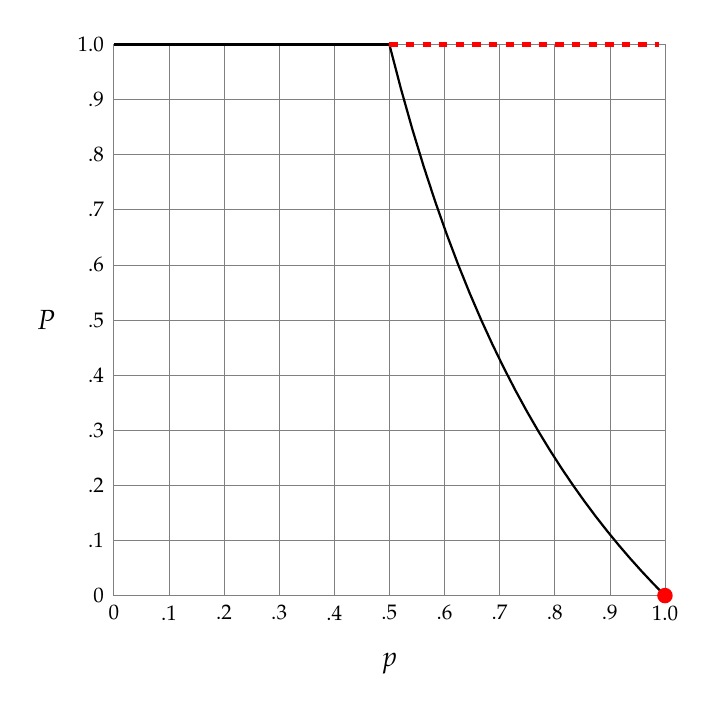
\begin{tikzpicture}[scale=7]
\draw[help lines,step=.1] (0,0) grid (1,1);
\foreach \x in {0,.1,.2,.3,.4,.5,.6,.7,.8,.9,1.0}
  \node[below] at (\x,0) {$\scriptstyle \x$};
\foreach \y in {0,.1,.2,.3,.4,.5,.6,.7,.8,.9,1.0}
  \node[left] at (0,\y) {$\scriptstyle \y$};
\draw[domain=0:.5,thick] plot (\x,1);
\draw[domain=.5:1,thick] plot (\x,{(1-\x)/\x});
\node at (.5,-3.5pt) {$p$};
\node at (-3.5pt,.5) {$P$};
\draw[ultra thick,red,dashed] (.5,1) -- +(.49,0);
\fill[red] (1,0) circle[radius=.4pt];
\end{tikzpicture}
\end{center}
\caption{הגרף של $P=\min(p/(1-p),1)$ עבור $p\in [0,1]$}\label{f.ruin2}
\end{figure}
עבור
$p=2/3, P=1/2$
ועבור
$p=1/2, P=1$.
זה מפתיע כי לא היינו מצפים שהחלקיק יחזור תמיד ל-%
$0$
אם כיוון הצעד נקבע על ידי הטלת מטבע הוגן! אנו זקוקים למטבע ממש לא-הוגן (הסתברות של "עץ" שווה ל-%
$2/3$)
כדי להשוות את הסיכויים לחזור ל-%
$0$
או לא.

\sml{}

\selectlanguage{english}
\begin{verbatim}
For probability = 0.2500:
Probability of reaching 0 = 1.0000
Proportion reaching 0     = 1.0000
For probability = 0.5000:
Probability of reaching 0 = 1.0000
Proportion reaching 0     = 0.9612
For probability = 0.6667:
Probability of reaching 0 = 0.5000
Proportion reaching 0     = 0.5043
For probability = 0.7500:
Probability of reaching 0 = 0.3333
Proportion reaching 0     = 0.3316
For probability = 0.8000:
Probability of reaching 0 = 0.2500
Proportion reaching 0     = 0.2502
\end{verbatim}
\selectlanguage{hebrew}

%%%%%%%%%%%%%%%%%%%%%%%%%%%%%%%%%%%%%%%%%%%%%%%%%%%%%%%%%%%%%

\begin{prob}{פשיטת הרגל של מהמר}{D}{(Gambler's ruin)}

חלקיק מוצב על ציר ה-%
$x$
במקום
$m\geq 1$.
בכל מקום על ציר ה-%
$x$
הוא יכול לצעוד צעד ימינה עם הסתברות
$p>1/2$
וצעד שמאלה עם הסתברות
$1-p$.

\que{1}
מה ההסתברות שהחלקיק יגיע למקום
$0$
בסופו של דבר?

\que{2} יהי 
$n>m$.
אם החלקיק מגיע למקום 
$0$
או למקום
$n$
הוא מפסיק לצעוד (איור%
~\ref{f.ruin3}).
מה ההסתברות שהחלקיק יגיע למקום 
$0$?
מה ההסתברות שהחלקיק יגיע למקום
$n$?
\begin{figure}[tb]
\begin{center}
\begin{tikzpicture}[scale=1.5]
\draw (0,0) -- (6,0);
\foreach \x in {0,1,2,3,4,5,6} {
  \draw (\x,0) -- +(0,4pt);
  \node at (\x,-10pt) { $\x$ };
}
\node at (2,-20pt) {$m$};
\node at (6,-20pt) {$n$};
\draw[fill] (2,5mm) circle[radius=.5pt];
\draw[->] (2,5mm) -- node[above] {$1/3$} (1,5mm);
\draw[->] (2,5mm) -- node[above] {$2/3$} (3,5mm);
\end{tikzpicture}
\end{center}
\caption{האם החלקיק יכול לחזור ל-%
$0$ (ציר סופי)?}
\label{f.ruin3}
\end{figure}

\textbf{הערה:} 
בעיה%
~$35$
מייצגת מהמר המשחק עם כמות סופית של כסף נגד קזינו עם כמות בלתי מוגבלת של כסף. הבעיה מבקשת את ההסתברות שהמהמר יפסיד את כל כספו. בעיה~%
$36(2)$
שואלת על מהמר אחד עם 
$m$
שמשחק נגד מהמר שני עם 
$n-m$.
הבעיה מבקשת את ההסתברויות ש%
\textbf{אחד}
מהם מפסיד את כל כספו לשני.
\end{prob}

\solution{}

הפתרון מבוסס על
\L{\cite[Chapter~2, Example~4m]{ross}}.

נסמן ב-%
$P(i,j)$
את ההסתברות שהחלקיק מגיע ל-%
$i$
מ-%
$j$.

\ans{1}
ראינו בפתרון לבעיה%
~$35$
שעבור
$p>1/2$
(כאן נתון), אם חלקיק נמצא במקום 
$1$
ההסתברות שלו להגיע ל-%
$0$
היא
$r=(1-p)/p$.
הסתברות זו לא תלויה במקום האבסולוטי של החלקיק ולכן:
\[
P(i,j) = P(i+k,k+1) = P(i-k,j-k)\,,
\]
ו-%
\begin{equation}
P(0,m)=P(m-1,m)P(m-2,m-1)\cdots P(1,2)P(0,1)=r^m\,.
\end{equation}

\ans{2} 
סמן בקיצור
$P_i=P(n,i)$
וחשב את
$P_i$:
\begin{eqn}
P_i &=& pP_{i+1} + (1-p)P_{i-1}\\
%pP_{i+1}&=&1\cdot P_i - (1-p)P_{i-1}\\
pP_{i+1}&=&(p+(1-p))P_i - (1-p)P_{i-1}\\
p(P_{i+1}-P_i)&=&(1-p)(P_i-P_{i-1})\\
P_{i+1}-P_i&=&r(P_i-P_{i-1})\,.
\end{eqn}
$P_0=0$ 
כי אם החלקיק נמצא ב-%
$0$
הוא מפסיק לצעוד. לכן:
\begin{eqn}
P_2 - P_1 &=& r(P_1 - P_0) = rP_1\\
P_3 - P_2 &=& r(P_2 - P_1) = r^2P_1\\
\cdots &=&\cdots\\
P_i - P_{i-1} &=& r(P_{i-1} - P_{i-2}) = r^{i-1}P_1\,.
\end{eqn}
רוב הגורמים בצד השמאלי מצטמצמים כאשר מחברים את המשוואות:
\begin{eqnlabels}
\nonumber{}P_i - P_1 &=& P_1\sum_{j=2}^{i}r^{j-1}\\
\nonumber{}&=& P_1 + P_1\sum_{j=2}^{i}r^{j-1} - P_1 \\
\label{eq.ruin0}P_i&=& P_1\sum_{j=0}^{i-1}r^j =P_1\left(\frac{1-r^i}{1-r}\right)\,.
\end{eqnlabels}
אם חלקיק נמצא ב-%
$n$
הוא כבר נמצא ב-%
$n$
כך ש-%
$P_n=1$:
\begin{eqnlabels}
\nonumber{}1 &=& P_1\left(\frac{1-r^n}{1-r}\right)\\
\label{eq.ruin00}P_1 &=& \left(\frac{1-r}{1-r^n}\right)\,.
\end{eqnlabels}
ממשוואות%
~\ref{eq.ruin0}, \ref{eq.ruin00}:
\begin{equation}
\label{eq.ruin1}P(n,i) = \left(\frac{1-r^{i}}{1-r^n}\right)\,.
\end{equation}
בהוכחה סימטרית שמחליפה את
$p$
ו-%
$1-p$):
\begin{equation}
\label{eq.ruin2}P(0,i) = \left(\frac{1-(1/r)^{n-i}}{1-(1/r)^{n}}\right)\,.
\end{equation}
הקורא מוזמן להראות שהסכום של משוואות
~\ref{eq.ruin1},~\ref{eq.ruin2}
הוא $1$ כלומר שמובטח שאחד המהמרים ינצח והשני יפסיד. עבור
$m=1, n=3, p=2/3$:
\begin{eqn}
P(0,1) &=& \left(\frac{1-\left(\frac{1}{2}\right)^{1}}{1-\left(\frac{1}{2}\right)^{3}}\right)=\frac{4}{7}\\
P(3,1) &=& \left(\frac{1-2^{2}}{1-2^{3}}\right)=\frac{3}{7}\,.
\end{eqn}

\sml{}
\selectlanguage{english}
\begin{verbatim}
For probability = 0.6667:
Probability of reaching (0,10) from 1 = (0.4995,0.5005)
Proportion reaching     (0,10) from 1 = (0.5056,0.4944)
Probability of reaching (0,10) from 4 = (0.0616,0.9384)
Proportion reaching     (0,10) from 4 = (0.0643,0.9357)
Probability of reaching (0,10) from 6 = (0.0147,0.9853)
Proportion reaching     (0,10) from 6 = (0.0123,0.9877)
\end{verbatim}

\begin{verbatim}
For probability = 0.7500:
Probability of reaching (0,10) from 1 = (0.3333,0.6667)
Proportion reaching     (0,10) from 1 = (0.3395,0.6605)
Probability of reaching (0,10) from 4 = (0.0123,0.9877)
Proportion reaching     (0,10) from 4 = (0.0115,0.9885)
Probability of reaching (0,10) from 6 = (0.0014,0.9986)
Proportion reaching     (0,10) from 6 = (0.0015,0.9985)
\end{verbatim}
\selectlanguage{hebrew}
ככל שלמהמר בצד שמאל יש יותר והסתברות גבוהה היותר לזכות בכל צעד, כך ההסתברות שלו לניצחון גדלה.

\textbf{גרף של הצעדים}

איור%
~\ref{f.plot}
נוצר בעזרת ספריית 
\L{\texttt{matplotlib}}
של
\L{Python}.
קור המקור מופיע בקובץ:
\begin{center}
\L{\texttt{36-gamblers-ruin-plot.py}}
\end{center}

\begin{figure}
\begin{center}
% This file was created with tikzplotlib v0.10.1.
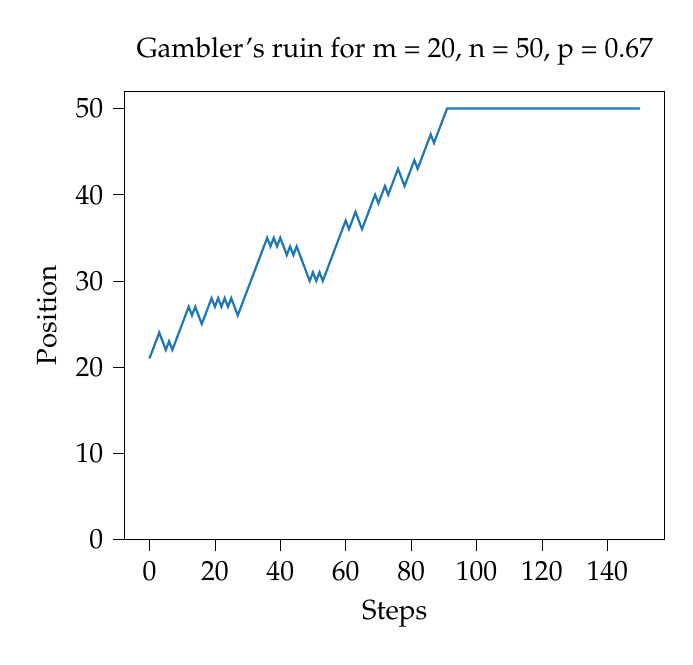
\begin{tikzpicture}

\definecolor{darkgray176}{RGB}{176,176,176}
\definecolor{steelblue31119180}{RGB}{31,119,180}

\begin{axis}[
tick align=outside,
tick pos=left,
title={Gambler's ruin for m = 20, n = 50, p = 0.67},
x grid style={darkgray176},
xlabel={Steps},
xmin=-7.5, xmax=157.5,
xtick style={color=black},
y grid style={darkgray176},
ylabel={Position},
ymin=0, ymax=52,
ytick style={color=black}
]
\addplot [thick, steelblue31119180]
table {%
0 21
1 22
2 23
3 24
4 23
5 22
6 23
7 22
8 23
9 24
10 25
11 26
12 27
13 26
14 27
15 26
16 25
17 26
18 27
19 28
20 27
21 28
22 27
23 28
24 27
25 28
26 27
27 26
28 27
29 28
30 29
31 30
32 31
33 32
34 33
35 34
36 35
37 34
38 35
39 34
40 35
41 34
42 33
43 34
44 33
45 34
46 33
47 32
48 31
49 30
50 31
51 30
52 31
53 30
54 31
55 32
56 33
57 34
58 35
59 36
60 37
61 36
62 37
63 38
64 37
65 36
66 37
67 38
68 39
69 40
70 39
71 40
72 41
73 40
74 41
75 42
76 43
77 42
78 41
79 42
80 43
81 44
82 43
83 44
84 45
85 46
86 47
87 46
88 47
89 48
90 49
91 50
92 50
93 50
94 50
95 50
96 50
97 50
98 50
99 50
100 50
101 50
102 50
103 50
104 50
105 50
106 50
107 50
108 50
109 50
110 50
111 50
112 50
113 50
114 50
115 50
116 50
117 50
118 50
119 50
120 50
121 50
122 50
123 50
124 50
125 50
126 50
127 50
128 50
129 50
130 50
131 50
132 50
133 50
134 50
135 50
136 50
137 50
138 50
139 50
140 50
141 50
142 50
143 50
144 50
145 50
146 50
147 50
148 50
149 50
150 50
};
\end{axis}

\end{tikzpicture}

\end{center}
\caption{פשיטת רגל של מהמר $m = 20, n = 50, p = 0.67$}\label{f.plot}
\end{figure}

%%%%%%%%%%%%%%%%%%%%%%%%%%%%%%%%%%%%%%%%%%%%%%%%%%%%%%%%%%%%%

\begin{prob}{משחק נועז או משחק זהיר}{}{(Bold play vs. cautious play)}

משחק הרולט מתואר בבעיה%
~$7$
(עמוד%
\pageref{p.roulette}).

איזו מהאסטרגיות שלהלן עדיפה?
\begin{enumerate}
\item 
משחק נועז: להמר $20$ בסיבוב אחד.
\item
משחק זהיר: להמר $1$ בכל סיבוב עד שאתה זוכה או מפסיד $20$.
\end{enumerate}
\textbf{רמז:} 
השתמש בתוצאות של בעיה%
~$36$.
\end{prob}

\solution{}

ההסתברות לנצח במשחק נועז היא
$18/38\approx 0.4737$.

משחק זהיר הוא בעיית "פשיטת רגל של מהמר" (בעיה%
~$36$):
אתה מתחיל עם 
$20$
ומשחק עד שאתה מגיע ל-%
$40$
(הרווחת 
$20$)
או אד שאתה מגיע ל-%
$0$
(הפסדת
$20$).
ההסתברות לנצח במשחק זהיר נתונה על ידי משוואה%
~\ref{eq.ruin1}
עם
$p=18/38$
ו-%
$1-p=20/38$
כך ש-%
$r=20/18$:
\begin{eqnarray*}
r&=&\frac{20}{38}\Big /\frac{18}{38}=\frac{20}{18}\\
P(40,20) &=&
\frac{1-(20/18)^{20}}{1-(20/18)^{40}}\approx 0.1084\,.
\end{eqnarray*}
ברור שמשחק נועז עדיף על משחק זהיר.

\L{Mosteller}
מביא הסבר איטואטיבי: הימור בסיבובים רבים חושף את המהמר לאפשרות שהקזינו מצנח אם הכדור נוחת בכיס ירוק עם הסתברות של
$2/38$.

\sml{}
\selectlanguage{english}
\begin{verbatim}
Probability of bold wins     = 0.4737
Proportion bold wins         = 0.4677
Probability of cautious wins = 0.1084
Proportion cautious wins     = 0.1094
\end{verbatim}
\selectlanguage{hebrew}

%%%%%%%%%%%%%%%%%%%%%%%%%%%%%%%%%%%%%%%%%%%%%%%%%%%%%%%%%%%%%

\refstepcounter{problem}

%%%%%%%%%%%%%%%%%%%%%%%%%%%%%%%%%%%%%%%%%%%%%%%%%%%%%%%%%%%%%

\begin{prob}{הכימאי המגושם}{}{(The clumsy chemist)}

נתון מספר רב של מקלות מזכוכית באורף 
$1$.
קצה אחד צבוע באדום (משובץ) ושני בכחול (מנוקד). כאשר זורקים אותם על הרצפה כל אחד נשבר לשלושה חלקים עם התפלגות אחידה של האורכים
(\ref{f.rod1}).
מה התוחלת של אורכו של החלק בקצה הכחול?

\textbf{רמז:}
במקום מקלות ישרים הנח שקבלת טבעות זכוכית (ללא סימנים) שגם הם נשברים לשלושה חלקים
(\ref{f.rod2}).

\begin{figure}[tb]
\begin{center}
\begin{subfigure}{.4\textwidth}
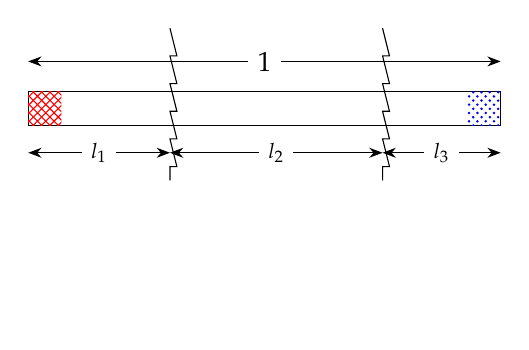
\begin{tikzpicture}
\draw (0,0) -- ++(6,0) -- ++(0,12pt) -- ++(-6,0) -- cycle;
\fill[pattern=crosshatch,pattern color=red]
  (0,0) rectangle +(12pt,12pt);
\fill[pattern=crosshatch dots,pattern color=blue]
  (6,0) rectangle +(-12pt,12pt);
\draw[<->] (0,23pt) --
  node[fill=white] {$1$} ++(6,0);
\draw[decorate,decoration=saw] (1.8,35pt) -- +(0,-55pt);
\draw[decorate,decoration=saw] (4.5,35pt) -- +(0,-55pt);
\draw[<->] (0,-10pt) --
  node[fill=white] {$\scriptstyle l_1$} (1.8,-10pt);
\draw[<->] (1.8,-10pt) --
  node[fill=white] {$\scriptstyle l_2$} (4.5,-10pt);
\draw[<->] (4.5,-10pt) --
  node[fill=white] {$\scriptstyle l_3$} (6,-10pt);
\path (0,-1) rectangle +(2,-1.5);
\end{tikzpicture}
\caption{חלוקת מקל לשלושה חלקים}\label{f.rod1}
\end{subfigure}
\hspace{3em}
\begin{subfigure}[b]{.4\textwidth}
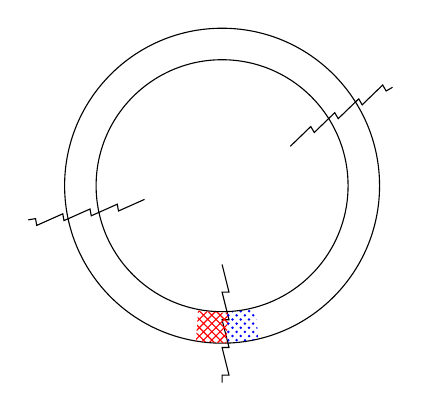
\begin{tikzpicture}
\draw (0,0) circle[radius=2];
\draw (0,0) circle[radius=1.6];
\draw[decorate,decoration=saw] (30:1) -- +(30:1.5);
\draw[decorate,decoration=saw] (190:1) -- +(190:1.5);
\draw[decorate,decoration=saw] (-90:1) -- +(-90:1.5);
\node[rotate=-4,minimum width=11pt,minimum height=11pt,
      pattern=crosshatch,pattern color=red]
  at (-94:1.8) {};
\node[rotate=6,minimum width=11pt,minimum height=11pt,
      pattern=crosshatch dots, pattern color=blue]
  at (-82:1.8) {};
\end{tikzpicture}
\caption{חלוקת טבעת לשלושה חלקים}\label{f.rod2}
\end{subfigure}
\end{center}
\end{figure}
\end{prob}

\solution{1}

אין סימטריה במקלות כי הקצוות שונים מהחלק האמצעי. אולם הטבעת סימטרית ולכן ההתפלגויות של שלושת החלקים יהיו אחידות עם תוחלת
$1/3$.
על ידי צביעת אחת מנקודות השבירה כפי שמופיע ב%
\ref{f.rod2},
הבעיה הופכת להיות זהה לבעיית המקל כך שההתפלגויות זהות. לכן התוחלת של אורכי החלקים היא גם
$1/3$.

\solution{2}

פתרון אלגנטי זה מבוסס על
\L{\cite{stack-rods}}.

נניח שהמקל מייצג את קטע הקו 
$(0,1)$.
המקל נשבר בשני מקומות שניתן לייצג על ידי שני משתנים אקראיים בלתי-תלויים עם התפלגות אחידה
$X,Y\in (0,1)$.
נחשב את ההסתברות
$P(|X-Y|>a)$.

טבלה%
~\ref{t.rods}
מראה נקודות 
$(x,y)$
כאשר
$x,y \in \{0.0, 0.1, 0.2, \ldots, 0.9\}$
והנקודה העשרונית הושמטה. הערכים בטבלה הם
$|X-Y|$.
עבור
$a=0.6$
הערכים למעלה משמאל (מודגשים) והערכים למטה מימין (מודגשים) הם התוצאות שמגדירות את
$P(|X-Y|>a)$:
\[
G(a)=P(|X-Y|>a)=2\cdot \frac{1}{2}(1-a)(1-a)=(1-a)^2\,.
\]
אנחנו מעוניינים המשלים:
\[
F(a)=1-G(a)=P(|X-Y|<a)=1-(1-a)^2=2a-a^2\,.
\]
זאת ההתפלגות ההסתברות המצטברת 
(CPD)
עבור הקטע
$(0,1)$. 
\begin{table}[bt]
\[
\begin{array}{c}
\quad\\\\\\
a\\\\
\quad\\
y\\
\quad\\\quad\\\quad\\\quad
\end{array}
\begin{array}{|c|cccccccccc|}
\multicolumn{11}{l}{\qquad \qquad \qquad a}\\
\hline
9& \mathbf{9} & \mathbf{8} & \mathbf{7} & \mathbf{6} & 5 & 4 & 3 & 2 & 1 & 0  \\
8& \mathbf{8} & \mathbf{7} & \mathbf{6} & 5 & 4 & 3 & 2 & 1 & 0 & 1  \\
7& \mathbf{7} & \mathbf{6} & 5 & 4 & 3 & 2 & 1 & 0 & 1 & 2  \\
6& \mathbf{6} & 5 & 4 & 3 & 2 & 1 & 0 & 1 & 2 & 3  \\
5& 5 & 4 & 3 & 2 & 1 & 0 & 1 & 2 & 3 & 4  \\
4& 4 & 3 & 2 & 1 & 0 & 1 & 2 & 3 & 4 & 5  \\
3& 3 & 2 & 1 & 0 & 1 & 2 & 3 & 4 & 5 & \mathbf{6}  \\
2& 2 & 1 & 0 & 1 & 2 & 3 & 4 & 5 & \mathbf{6} & \mathbf{7}  \\
1& 1 & 0 & 1 & 2 & 3 & 4 & 5 & \mathbf{6} & \mathbf{7} & \mathbf{8}  \\
0& 0 & 1 & 2 & 3 & 4 & 5 & \mathbf{6} & \mathbf{7} & \mathbf{8} & \mathbf{9}  \\
\hline
&0 & 1 & 2 & 3 & 4 & 5 & 6 & 7 & 8 & 9  \\
\hline
\multicolumn{11}{c}{\quad \quad x\quad\quad\quad a}
\end{array}
\begin{array}{c}
\\\\\\
a\\\\
\end{array}
\]
\caption{התפלגות נקודות השבירה ב-%
$(0,1)\times (0,1)$}\label{t.rods}
\end{table}
ניתן לקבל את פונקציית ההסתברות הצפיפות
(PDF)
על ידי גזירת ה-%
CDP:
\[
f(a)=P(|X-Y|=a)= \frac{d}{da}F(a) =
  \frac{d}{da}(2a-a^2)=2(1-a)\,.
\]
התוחלת היא האינטגרל של ה-%
PDF
כפול הערך:
\[
E(|X-Y|)= \int_{0}^{1} a\cdot2(1-a)\, da=
  2\left.\left(\frac{a^2}{2}-\frac{a^3}{3}\right)\right|_0^1=\frac{1}{3}\,.
\]

\sml{}
\selectlanguage{english}
\begin{verbatim}
Expectation of length of right piece = 0.3333
Average length of right piece        = 0.3359
\end{verbatim}
\selectlanguage{hebrew}

%%%%%%%%%%%%%%%%%%%%%%%%%%%%%%%%%%%%%%%%%%%%%%%%%%%%%%%%%%%%%

\begin{prob}{האס הראשון}{}{(The first ace)}

חלק קלפים מחפיסה מעורבת היטב עד שמופיע אס. מה התוחלת של מספר הקלפים שיש לחלק?

\textbf{רמז:}
חשוב על חפיסת קלפים ללא האסים מסודרת בשורה.
\end{prob}

\solution{}
הקלפים הם כמו "מקל" באורך 
$48$
"שנשבר" על ידי 
$4$
ל-%
$5$
חלקים. הפתרון של בעיה%
~$39$
מתאים גם כאן והתוחלת של חלק היא
$48/5=9.6$.

\newpage

\sml{}
\selectlanguage{english}
\begin{verbatim}
Expectation of first ace = 9.6000
Average first ace        = 9.5805
\end{verbatim}
\selectlanguage{hebrew}

%%%%%%%%%%%%%%%%%%%%%%%%%%%%%%%%%%%%%%%%%%%%%%%%%%%%%%%%%%%%%


% !TeX root = mos-en.tex

%%%%%%%%%%%%%%%%%%%%%%%%%%%%%%%%%%%%%%%%%%%%%%%%%%%%%%%%%%%%%%%%

\begin{prob}{Should you sample with or without replacement?\annotate{D}}
Urn $A$ contains $2$ red balls and $1$ green ball, and urn $B$ contains $101$ red balls and $100$ green balls. An urn is chosen at random and two balls are randomly drawn from the selected urn. You win if you correctly identify whether the selected urn was $A$ or $B$.

Compute the probabilities of winning for each of the following rules and decide which gives you the highest probability of winning.

\que{1} The first ball is replaced before the second drawing.

\que{2} The first ball is not replaced before the second drawing.

\que{3} After the first ball is drawn you can decide whether it will be replaced or not.

\textbf{Hint:} When computing probabilities:
\[
\disfrac{101}{201}\approx \disfrac{100}{201} \approx \disfrac{100}{200} \approx \disfrac{1}{2}\,.
\]
\end{prob}

\solution{}

There are four outcomes which we denote by $RR, RG, GR, GG$. For each rule compute the conditional probabilities of the four outcomes given that urn $A$ or urn $B$ was selected initially. These probabilities are multiplied by $1/2$ to take into account the random selection of a urn.

\ans{1} Drawing with replacement:
\[
\renewcommand*{\arraystretch}{1.5}
\begin{array}{lcccc}
P(RR|A) &=& \frac{2}{3} \cdot \frac{2}{3} &=& \frac{4}{9}\\
P(RR|B) &=& \frac{1}{2} \cdot \frac{1}{2} &=& \frac{1}{4}\\
\hline
P(RG|A) &=& \frac{2}{3} \cdot \frac{1}{3} &=& \frac{2}{9}\\
P(RG|B) &=& \frac{1}{2} \cdot \frac{1}{2} &=& \frac{1}{4}\\
\hline
P(GR|A) &=& \frac{1}{3} \cdot \frac{2}{3} &=& \frac{2}{9}\\
P(GR|B) &=& \frac{1}{2} \cdot \frac{1}{2} &=& \frac{1}{4}\\
\hline
P(GG|A) &=& \frac{1}{3} \cdot \frac{1}{3} &=& \frac{1}{9}\\
P(GG|B) &=& \frac{1}{2} \cdot \frac{1}{2} &=& \frac{1}{4}\end{array}
\]
If the outcome is $RR$ there is a higher probability that urn $A$ was selected ($4/9$) than that urn $B$ was selected ($1/4$); otherwise, there is a higher probability that urn $B$ was selected. Therefore:
\[
P(\textsf{winning})=\frac{1}{2}\left(\frac{4}{9} + \frac{1}{4}+ \frac{1}{4}+ \frac{1}{4}\right)=\disfrac{43}{72}\approx 0.5972\,.
\]

\ans{2} Drawing without replacement:
\[
\renewcommand*{\arraystretch}{1.5}
\begin{array}{lcccc}
P(RR|A) &=& \frac{2}{3} \cdot \frac{1}{2} &=& \frac{1}{3}\\
P(RR|B) &=& \frac{1}{2} \cdot \frac{1}{2} &=& \frac{1}{4}\\
\hline
P(RG|A) &=& \frac{2}{3} \cdot \frac{1}{2} &=& \frac{1}{3}\\
P(RG|B) &=& \frac{1}{2} \cdot \frac{1}{2} &=& \frac{1}{4}\\
\hline
P(GR|A) &=& \frac{1}{3} \cdot 1 &=& \frac{1}{3}\\
P(GR|B) &=& \frac{1}{2} \cdot \frac{1}{2} &=& \frac{1}{4}\\
\hline
P(GG|A) &=& \frac{1}{3} \cdot 0 &=& 0\\
P(GG|B) &=& \frac{1}{2} \cdot \frac{1}{2} &=& \frac{1}{4}
\end{array}
\]
If the outcome is $GG$ there is (of course!) a higher probability that urn $B$ was selected than that urn $A$ was selected; otherwise, there is a higher probability that urn $A$ was selected. Therefore:
\[
P(\textsf{winning})=\frac{1}{2}\left(\frac{1}{3} + \frac{1}{3}+ \frac{1}{3}+ \frac{1}{4}\right)=\frac{5}{8}=0.6250\,,
\]
which is greater than the probability of winning when sampling with replacement.

\ans{3} The decision is based on the outcome of the first draw.

If the first drawing is from urn $A$ the probabilities must be conditioned on the decision to sample with or without replacement. Drawing first from urn $B$ does not affect the probabilities because of the approximation in the hint.
\[
\renewcommand*{\arraystretch}{1.5}
\begin{array}{lcccc}
P(RR|A,w) &=& \frac{2}{3} \cdot \frac{2}{3} &=& \frac{4}{9}\\
P(RR|A,w/o) &=& \frac{2}{3} \cdot \frac{1}{2} &=& \frac{1}{3}\\
P(RR|B) &=& \frac{1}{2} \cdot \frac{1}{2} &=& \frac{1}{4}\\
\hline
P(RG|A,w) &=& \frac{2}{3} \cdot \frac{1}{3} &=& \frac{2}{9}\\
P(RG|A,w/o) &=& \frac{2}{3} \cdot \frac{1}{2} &=& \frac{1}{3}\\
P(RG|B) &=& \frac{1}{2} \cdot \frac{1}{2} &=& \frac{1}{4}\\
\hline
%\end{array}
%\]
%\[
%\renewcommand*{\arraystretch}{1.5}
%\begin{array}{lcccc}
P(GR|A,w) &=& \frac{1}{3} \cdot \frac{2}{3} &=& \frac{2}{9}\\
P(GR|A,w/o) &=& \frac{1}{3} \cdot 1 &=& \frac{1}{3}\\
P(GR|B) &=& \frac{1}{2} \cdot \frac{1}{2} &=& \frac{1}{4}\\
\hline
P(GG|A,w) &=& \frac{1}{3} \cdot \frac{1}{3} &=& \frac{1}{9}\\
P(GG|A,w/o) &=& \frac{1}{3} \cdot 0 &=&0\\
P(GG|B) &=& \frac{1}{2} \cdot \frac{1}{2} &=& \frac{1}{4}\\\end{array}
\]
If a red ball is drawn first then $\frac{4}{9}>\frac{1}{4}$ and $\frac{2}{9}<\frac{1}{4}$ with replacement, whereas $\frac{1}{3}>\frac{1}{4}$ and $\frac{1}{3}>\frac{1}{4}$ without replacement, so the second ball can help identify the urn only if the drawing is done \emph{with} replacement: urn $A$ if red, urn $B$ if green. Choose the draw with replacement and:
\[
P(\textsf{winning if red first})=\frac{1}{2}\left(\frac{4}{9}+\frac{1}{4}\right)=\frac{25}{72}\,.
\]
If a green ball is drawn first then $\frac{2}{9}<\frac{1}{4}$ and $\frac{1}{9}<\frac{1}{4}$ with replacement, whereas $\frac{1}{3}>\frac{1}{4}$ and $0<\frac{1}{4}$ without replacement, so the second ball can help identify the urn only if the drawing is done \emph{without} replacement: urn $A$ if red, urn $B$ if green. Choose the draw without replacement and:
\[
P(\textsf{winning if green first})=\frac{1}{2}\left(\frac{1}{3}+\frac{1}{4}\right)=\frac{7}{24}\,.
\]
The probability of winning is:
\[
P(\textsf{winning})=\frac{25}{72} + \frac{7}{24}=\frac{23}{36}\approx 0.6389\,.
\]
The highest probability of winning is obtained when the decision to draw with or without replacement depends on the result of the first draw.

\textbf{Simulation}
\begin{verbatim}
With replacement:
Expectation of winning = 0.5972
Average wins           = 0.5976
Without replacement:
Expectation of winning = 0.6250
Average wins           = 0.6207
Decide after first draw:
Expectation of winning = 0.6389
Average wins           = 0.6379
\end{verbatim}


%%%%%%%%%%%%%%%%%%%%%%%%%%%%%%%%%%%%%%%%%%%%%%%%%%%%%%%%%%%%%


\begin{prob}{The ballot box}
In an election there are two candidates $A$ and $B$.  $A$ receives $a$ votes and $B$ receives $b$ votes, $a>b$. The votes are counted one-by-one and the running totals $(a_i,b_i), 1\leq i \leq a+b$ are updated as each vote is counted. What is the probability that for at least one $i$, $a_i=b_i$?

\que{1} Solve for $a=3, b=2$ by listing $(a_i,b_i)$ for $1\leq i\leq 5$.

\que{2} Solve for all $a>b$.

\textbf{Hint 1:} What can you say about the identity of the candidate who leads until the \emph{first} tie occurs?

\textbf{Hint 2:} What is the significance of the first vote counted?
\end{prob}

\solution{}

\ans{1}
The number of arrangements of running totals is ${5\choose 2}={5\choose 3}=10$, because the positions of the votes for one candidate determine the positions of the votes for the other candidate. The following table lists the possible arrangements of the votes and of running totals with first ties emphasized:
\begin{center}
\begin{minipage}{.48\textwidth}
\[
\begin{array}{ccccc}
A & A & A & B & B\\
A & A & B & A & B\\
A & B & A & A & B\\
B & A & A & A & B\\%\hline
A & A & B & B & A\\
A & B & A & B & A\\
B & A & A & B & A\\%\hline
A & B & B & A & A\\
B & A & B & A & A\\%\hline
B & B & A & A & A
\end{array}
\]
\end{minipage}
\hspace{-4em}
\begin{minipage}{.48\textwidth}
\[
\begin{array}{rrrrr}
%(4,5)&
(1,0) & (2,0) & (3,0) & (3,1) & (3,2)\\
%(3,5)&
(1,0) & (2,0) & (2,1) & (3,1) & (3,2)\\
%(2,5)&
(1,0) & \mathbf{(1,1)} & (2,1) & (3,1) & (3,2)\\
%(1,5)&
(0,1) & \mathbf{(1,1)} & (2,1) & (3,1) & (3,2)\\%\hline
%(3,4)&
(1,0) & (2,0) & (2,1) & \mathbf{(2,2)} & (3,2)\\
%(2,4)&
(1,0) & \mathbf{(1,1)} & (2,1) & (2,2) & (3,2)\\
%(1,4)&
(0,1) & \mathbf{(1,1)} & (2,1) & (2,2) & (3,2)\\%\hline
%(2,3)&
(1,0) & \mathbf{(1,1)} & (1,2) & (2,2) & (3,2)\\
%(1,3)&
(0,1) & \mathbf{(1,1)} & (1,2) & (2,2) & (3,2)\\%\hline
%(1,2)&
(0,1) & (0,2) & (1,2) &  \mathbf{(2,2)} & (3,2)
\end{array}
\]
\end{minipage}
\end{center}
There are ties in all the arrangements except for the first two so:
\[
P(\textsf{tie occurs with}\;(3,2)\;\textsf{votes})=\disfrac{8}{10}=\disfrac{4}{5}\,.
\]

\ans{2} 
We begin the solution with a discussion on how to approach the second question. Here are some arrangements for $(a,b)=(3,2)$ votes until the \emph{first tie} occurs:
\[
\begin{array}{rrrrr|rrrrr}
\multicolumn{5}{c|}{A \;\textsf{leads until tie}} &
\multicolumn{5}{c}{B \;\textsf{leads until tie}}\\\hline
A & B &&& &B & A & & &\\
A & A & B & B && B & B & A & A&\\
\end{array}
\]
For every arrangement where $A$ leads until the first tie, there is a mirror image arrangement where $B$ leads until the first tie. The mirror image is obtained by exchanging all $A$'s and $B$'s.

Before the first tie one of the candidates must be leading. If the first vote counted is for $B$ there must be a tie later in the count since $a>b$. The probability that the first vote is for $B$ is:
\[
P(\textsf{first vote for}\;B)=\frac{b}{a+b}\,.
\]
By mirroring the positions of the votes, the number of sequences resulting in a tie that begin with a vote for $A$ is the same as the number of sequences resulting in a tie that begin with a vote for $B$. Therefore:
\[
P(\textsf{tie occurs})=2\cdot\frac{b}{a+b}\,.
\]
Check:
\[
P(\textsf{tie occurs with}\;(3,2)\;\textsf{votes})=2\cdot\frac{2}{2+3}=\frac{4}{5}\,.
\]

\textbf{Simulation}
\begin{verbatim}
For a =  3, b =  2:
Probability of a tie = 0.8000
Proportion of ties   = 0.8118
For a = 10, b =  8:
Probability of a tie = 0.8889
Proportion of ties   = 0.8977
For a = 20, b = 18:
Probability of a tie = 0.9474
Proportion of ties   = 0.9354
\end{verbatim}


%%%%%%%%%%%%%%%%%%%%%%%%%%%%%%%%%%%%%%%%%%%%%%%%%%%%%%%%%%%%%

\begin{prob}{Ties in matching pennies\annotate{D}}
Toss a pair of fair coins $N$ times, $N$ even, and keep count of how many times the parity is even (heads-heads or tails-tails) and how many times the parity is odd (heads-tails or tails-heads). What is the probability of obtaining a tie (not counting the $0-0$ tie at the start)?

\que{1} Solve for $N=4$ by writing out all the possible outcomes.

\que{2} Solve for $N=6$ by developing a formula for the probability.

\que{3} Develop a formula for arbitrary even $N$.

\que{4} Explain why the probability for the odd number $N+1$ is the same as the probability for the even number $N$.

\textbf{Hint:} Use the solution of Problem~22.
\end{prob}

\solution{}

\ans{1} Denote tosses with even parity by $E$ and tosses with odd parity by $O$. Ten out of the sixteen arrangements of tosses have ties (emphasized):
\begin{center}
\begin{tabular}{llllllll}
EEEE & EEEO & EEOE & \textbf{EEOO} & \textbf{EOEE} & \textbf{EOEO} &\textbf{EOOE} & \textbf{EOOO}\\
\textbf{OEEE} & \textbf{OEEO} & \textbf{OEOE} & \textbf{OEOO} & \textbf{OOEE} & OOEO&OOOE & OOOO
\end{tabular}
\end{center}

\ans{2}
By Problem~22:
\begin{equation}\label{eq.coins-ties}
P(\textsf{tie on toss}\;i)=
\left\{
\begin{array}{ll}
2i/N &\textsf{if}\; i\leq N/2\\
2(N-i)/N& \textsf{if}\; i\geq N/2\,,
\end{array}
\right.
\end{equation}
since the ballot box problem showed that the smaller value determines the probability.

The following computations are quite complex so we justify each step in detail.

The probability of $i$ evens is given by the binomial distribution:
\begin{equation}\label{eq.coins00}
P(i\;\textsf{evens})=\dischoose{N}{i} \left(\disfrac{1}{2}\right)^i \left(\disfrac{1}{2}\right)^{N-i}=\dischoose{N}{i} \left(\disfrac{1}{2}\right)^N =  2^{-N}\dischoose{N}{i}\,.
\end{equation}
The probability of a tie is the sum over $i$ of the probability of obtaining $i$ evens times the probability of a tie on the $i$th toss (Equation~\ref{eq.coins-ties}). For $N=6$:
\begin{equation}\label{eq.coins0}
P(\textsf{ties})=2\cdot 2^{-6}\left[
\frac{0}{6}\dischoose{6}{0} + \frac{1}{6}\dischoose{6}{1} +
\frac{2}{6}\dischoose{6}{2} + \frac{3}{6}\dischoose{6}{3} +
\frac{2}{6}\dischoose{6}{4} + \frac{1}{6}\dischoose{6}{5} +
\frac{0}{6}\dischoose{6}{6}
\right]\,.
\end{equation}
Equation~\ref{eq.coins1} follows from Equation~\ref{eq.coins0} by deleting the two zero terms, expressing the combinations as factorials, canceling $1/6$ from $6!$:
\begin{equation}\label{eq.coins1}
P(\textsf{ties})=2^{-5}\left[
1\cdot\disfrac{5!}{1!5!} + 2\cdot\disfrac{5!}{2!4!} +
3\cdot\disfrac{5!}{3!3!} + 2\cdot\disfrac{5!}{4!2!} +
1\cdot\disfrac{5!}{5!1!}
\right]\,.
\end{equation}
Equation~\ref{eq.coins2} is obtained by canceling $i$ from $i!$:
\begin{equation}\label{eq.coins2}
P(\textsf{ties})=2^{-5}\left[
\disfrac{5!}{1!5!} + \disfrac{5!}{1!4!} +
\disfrac{5!}{2!3!} + \disfrac{5!}{4!1!} +
\disfrac{5!}{5!1!}
\right]\,.
\end{equation}
To obtain Equation~\ref{eq.coins3} from Equation~\ref{eq.coins2} add and subtract  $\frac{5!}{3!2!}$:
\begin{equation}\label{eq.coins3}
P(\textsf{ties})=2^{-5}\left[
\left(\disfrac{5!}{1!5!} + \disfrac{5!}{1!4!} +
\disfrac{5!}{2!3!} + \disfrac{5!}{3!2!} +\disfrac{5!}{4!1!} +
\disfrac{5!}{5!1!}\right) - \disfrac{5!}{3!2!}
\right]\,.
\end{equation}
Equation~\ref{eq.coins4} results from  replacing $1!$ by $0!$:
\begin{equation}\label{eq.coins4}
P(\textsf{ties})=2^{-5}\left[
\left(\disfrac{5!}{0!5!} + \disfrac{5!}{1!4!} +
\disfrac{5!}{2!3!} + \disfrac{5!}{3!2!} +\disfrac{5!}{4!1!} +
\disfrac{5!}{5!0!}\right) - \disfrac{5!}{3!2!}
\right]\,.
\end{equation}
By expressing the factorials back as combinations we obtain  Equation~\ref{eq.coins5}:
\begin{equation}\label{eq.coins5}
P(\textsf{ties})=2^{-5}\left[
\dischoose{5}{0} + \dischoose{5}{1} +
\dischoose{5}{2} + \dischoose{5}{3} +
\dischoose{5}{4} + \dischoose{5}{5} - \dischoose{5}{3}
\right]\,.
\end{equation}
Finally, Equation~\ref{eq.coins6} results from the binomial theorem:
\begin{equation}\label{eq.coins6}
P(\textsf{ties})=2^{-5}\left(2^5 - 10\right)=\disfrac{11}{16}\approx 0.6875\,.
\end{equation}

\ans{3} Perform the same calculations as in \ansnc{2} but using arbitrary $N$. The result is:
\[
P(\textsf{ties})=2^{-N+1}\left[2^{N-1} - \dischoose{N-1}{N/2}\right]= 
\left[1 - \left.\dischoose{N-1}{N/2}\right/ 2^{N-1}\right]\,.
\]

\ans{4} The first tie on the $N+1$'st toss occurs only if the counts are nearly equal after the $N$th toss:
\[
\begin{array}{l}
((N/2)-1,(N/2)+1)\\((N/2),(N/2))\\((N/2)+1,(N/2)-1)
\end{array}
\]
but whatever the outcome of the final toss the counts will not be equal.

\textbf{Simulation}
\begin{verbatim}
For  4 tosses:
Probability of ties = 0.6250
Proportion of ties  = 0.6192
For  6 tosses:
Probability of ties = 0.6875
Proportion of ties  = 0.6900
For  7 tosses:
Probability of ties = 0.6875
Proportion of ties  = 0.6811
For 10 tosses:
Probability of ties = 0.7539
Proportion of ties  = 0.7559
For 20 tosses:
Probability of ties = 0.8238
Proportion of ties  = 0.8255
\end{verbatim}

%%%%%%%%%%%%%%%%%%%%%%%%%%%%%%%%%%%%%%%%%%%%%%%%%%%%%%%%%%%%%

\refstepcounter{problem} % 24. The unfair subway

%%%%%%%%%%%%%%%%%%%%%%%%%%%%%%%%%%%%%%%%%%%%%%%%%%%%%%%%%%%%%



\begin{prob}{Lengths of random chords}
Select a random chord in the unit circle. What is the probability that the length of the chord is greater than $1$?

To solve the problem you first have to decide what ``select a random chord'' means. Solve the problem for each of the following possibilities:

\que{1} The distance of the chord from the center is uniformly distributed.

\que{2} The midpoint of the chord is uniformly distributed within the circle.

\que{3} The endpoints of the chord are uniformly distributed on the circumference of the circle.
\end{prob}

\solution{}

\ans{1} A chord is larger than the radius if it is closer to the center than a chord of length $1$. Let $\overline{AB}$ be a chord of length $1$ and construct the altitude $\overline{OH}$ from the center $O$ to the chord (Figure~\ref{f.chord1}). Since $\triangle AOB$ is equilateral, $\triangle OHB$ is a right triangle and the length of the altitude is:
\[
h = \sin \frac{\pi}{3} = \frac{\sqrt{3}}{2}\,.
\]
Let $d$ be the distance of a chord $\overline{DE}$ from the center. By assumption $d$ is uniformly distributed in $(0,1)$ so: 
\[
P(\overline{DE}>1)=P(d<h)=\disfrac{h}{1}=\frac{\sqrt{3}}{2} \approx 0.866\,.
\]
\begin{figure}[tb]
\begin{center}
\begin{subfigure}[t]{.41\textwidth}
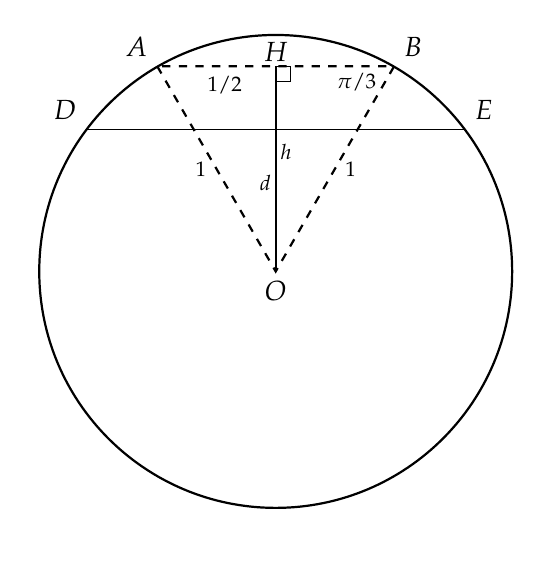
\begin{tikzpicture}[scale=.9]
\coordinate (O) at (0,0) node[below] {$O$};
\node (hexagon) [minimum size=6cm,regular polygon,
                 regular polygon sides=6] at (O) {};
\node[name path=circle,draw,thick,circle through=(hexagon.corner 1)] at (O) {};
\draw[thick,dashed] (hexagon.corner 2) -- 
  node[left] {$\scriptstyle 1$} (O) --
  node[right] {$\scriptstyle 1$} (hexagon.corner 1) -- cycle;
\node[above left] at (hexagon.corner 2) {$A$};
\node[above right] at (hexagon.corner 1) {$B$};
\coordinate (H) at (O |- hexagon.corner 1);
\node[above,yshift=-2pt] at (H) {$H$};
\draw[thick] (O) -- 
  node[right,xshift=-2pt,yshift=6pt] {$\scriptstyle h$} 
  node[left,xshift=2pt,yshift=-5pt] {$\scriptstyle d$}
  (H);
\draw[rotate=-90] (H) rectangle +(6pt,6pt);
\node[below left,xshift=-3pt,yshift=1pt] at 
  (hexagon.corner 1) {$\scriptstyle \pi/3$};
\path (hexagon.corner 2) -- 
  node[below,xshift=3pt] {$\scriptstyle 1/2$} (H) --
  (hexagon.corner 1);
\node[xshift=15mm,yshift=-8mm]  at (hexagon.corner 4)
  {};
\path[name path=chord] (-3.5,2) -- +(7,0);
\path [name intersections={of=circle and chord,by={E,D}}];
\draw (D) node[above left] {$D$} -- (E) node[above right] {$E$};
\end{tikzpicture}
\caption{Distance of chord from center uniformly distributed in $(0,1)$}\label{f.chord1}
\end{subfigure}
\hspace{3em}
\begin{subfigure}[t]{.45\textwidth}
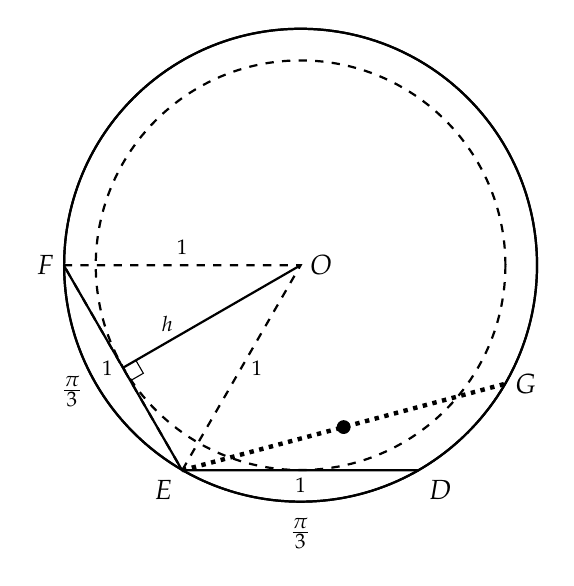
\begin{tikzpicture}[scale=.9]
\coordinate (O) at (0,0) node[right] {$O$};
\node (hexagon) [minimum size=6cm,regular polygon,
                 regular polygon sides=6] at (O) {};
\node[draw,thick,name path=circle,
      circle through=(hexagon.corner 1)] at (O) {};
\draw[thick,dashed] (hexagon.corner 3) -- 
  node[above] {$\scriptstyle 1$} (O) --
  node[right] {$\scriptstyle 1$} (hexagon.corner 4) -- cycle;
\coordinate (H) at ($(hexagon.corner 3)!.5!(hexagon.corner 4)$);
\draw[thick] (O) -- 
  node[above,near end] {$\scriptstyle h$} (H);
\draw[rotate=-60] (H) rectangle +(6pt,6pt);
\node[draw,thick,dashed,circle through=(H)] at (O) {};
\node[left]        at (hexagon.corner 3) {$F$};
\node[below left]  at (hexagon.corner 4) {$E$};
\node[xshift=-14mm,yshift=10mm]  at (hexagon.corner 4)
  {$\frac{\pi}{3}$};
\node[xshift=15mm,yshift=-8mm]  at (hexagon.corner 4)
  {$\frac{\pi}{3}$};
\node[below right] at (hexagon.corner 5) {$D$};
\draw[thick]  (hexagon.corner 3) --
     node[left] {$\scriptstyle 1$} (hexagon.corner 4) --
     node[below,yshift=1pt] {$\scriptstyle 1$}
     (hexagon.corner 5);
\node[draw,thick,name path=circle,
      circle through=(hexagon.corner 1)] at (O) {};
\path[name path=chord] (hexagon.corner 4) -- +(15:5);
\path [name intersections={of=circle and chord,by={K,L}}];
\node[right] at (L) {$G$};
\draw[ultra thick,dotted] (hexagon.corner 4) -- (L);
\coordinate (center) at ($(hexagon.corner 4)!.5!(L)$);
\vertex{center};
\end{tikzpicture}
\caption{Midpoint of chord uniformly distributed within the circle and endpoints of chord uniformly distributed on the circumference}\label{f.chord2}
\end{subfigure}
\end{center}
\end{figure}

\ans{2}
Construct a circle with center $O$ and radius $h$, where $h$ is the length of the altitude to a chord of length $1$. A tangent to any point on this circle will be a chord $\overline{FE}$ whose length is $1$. Any chord $\overline{EG}$ whose midpoint is within this circle will have a length greater than $1$ (Figure~\ref{f.chord2}). The probability that the length of the chord is greater than $1$ is therefore the ratio of the areas of the two circles:
\[
P(\overline{EG}>1)=\frac{\pi \cdot h^2}{\pi \cdot 1^2}=h^2=\frac{3}{4}\,.
\]
This is the square of the probability computed in the previous question.

\ans{3}
Choose an arbitrary point on the circumference of the unit circle ($E$ in Figure~\ref{f.chord2}). Any other point on the circumference (such as $G$ in the Figure) determines a chord whose length is greater than one unless that point falls on the arcs $\widehat{EF}$ or $\widehat{ED}$. The probability is therefore the ratio of the arc $\widehat{FD}$ to the circumference of the unit circle:
\[
P(\overline{EG}>1)=\frac{(2\pi-(2\pi/3))\cdot 1}{2\pi \cdot 1}=\frac{2}{3}\,.
\]

\textbf{Simulation}

The simulation is for choosing two random points on the circumference.
\begin{verbatim}
Probability of long chords = 0.6667
Proportion of long chords  = 0.6627
\end{verbatim}

%%%%%%%%%%%%%%%%%%%%%%%%%%%%%%%%%%%%%%%%%%%%%%%%%%%%%%%%%%%%%

\begin{prob}{The hurried duelers}
$A$ and $B$ arrive at a meeting point at a random time with uniform distribution within a one-hour period. If $A$ arrives first and $B$ does not arrive within $5$ minutes, $A$ leaves. Similarly if $B$ arrives first and $A$ does not arrive within $5$ minutes, $B$ leaves. What is the probability that they meet?

Time within the one-hour period is \emph{continuous} in the range $[0,1]$, that is, you cannot \emph{count} a discrete number of minutes or seconds to compute probabilities. You can compute the probabilities of \emph{durations}.

\textbf{Hint:} Draw a graph with $A$'s time of arrival as the the $x$-axis and $B$'s time of arrival as the $y$-axis.
\end{prob}

\solution{}

Without loss of generality assume that $A$ arrives first. If $A$ arrives at $t_A=0$ and if $B$ arrives before $t_B=5/60$ they meet, otherwise they do not. This is shown in Figure~\ref{f.duel} by the small square at the origin.
\begin{figure}[tb]
\begin{center}
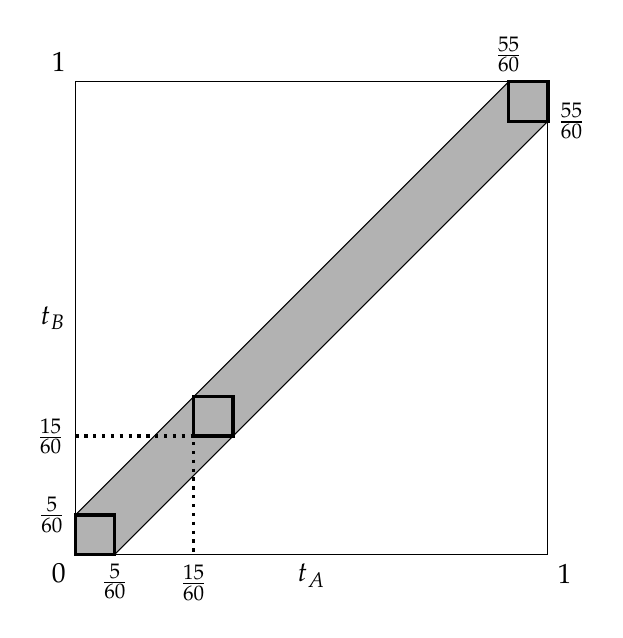
\begin{tikzpicture}
\draw (0,0) -- node[below] {$t_A$} (6,0) -- (6,6) -- (0,6) -- node[left] {$t_B$} cycle;
\node[below left]  at (0,0) {$0$};
\node[below right] at (6,0) {$1$};
\node[above left]  at (0,6) {$1$};
\draw[fill=white!70!black]
  (0,0) -- 
  (.5,0) node[below] {$\frac{5}{60}$} -- 
  (6,5.5) node[right] {$\frac{55}{60}$} --
  (6,6) -- (5.5,6) node[above] {$\frac{55}{60}$} --
  (0,.5) node[left] {$\frac{5}{60}$} -- cycle;
\draw[very thick] (0,0) -- (.5,0) -- (.5,.5) -- (0,.5) -- cycle;
\draw[very thick] (1.5,1.5) -- ++(.5,0) -- ++(0,.5) --
  ++(-.5,0) -- cycle;
\draw[very thick] (5.5,5.5) -- ++(.5,0) -- ++(0,.5) --
  ++(-.5,0) -- cycle;
\draw[very thick,dotted] (0,1.5) node[left] {$\frac{15}{60}$} --
  (1.5,1.5) -- (1.5,0) node[below] {$\frac{15}{60}$};
\end{tikzpicture}
\end{center}
\caption{Times that ensure a meeting between $A$ and $B$}\label{f.duel}
\end{figure}
If $A$ arrives later then $B$ also has to arrive later by the same amount; for example, if $A$ arrives at $t_A=15$, $B$ must arrive between $t_B=15$ and $t_B=20$. Therefore, the meeting will take place during a square of time obtained by moving the square by $15$ from $(0,0)$ to $(15/60,15/60)$.

The probability of a meeting is the ratio of the area of the graph colored gray to the area of the large square. It is easier to compute the complement which is the ratio of the area of the two white triangles to the area of the large square:
\begin{eqn}
P(A,B\;\textsf{meet}) &=& 1- P(A,B\;\textsf{don't meet})\\
&=&1- 2\cdot \left(\frac{1}{2}\cdot \frac{55}{60}\cdot \frac{55}{60}\right)=\frac{23}{144}\approx 0.1597\,.
\end{eqn}

\textbf{Simulation}
\begin{verbatim}
Probability of meeting   = 0.1597
Proportion of meetings   = 0.1549
\end{verbatim}

%%%%%%%%%%%%%%%%%%%%%%%%%%%%%%%%%%%%%%%%%%%%%%%%%%%%%%%%%%%%%

\begin{prob}{Catching the cautious counterfeiter}

There are $n$ boxes each with $n$ coins one of which is counterfeit. Draw one coin from each box and test it to determine whether it is counterfeit or genuine. What is the probability that all the coins that are drawn are are real?

\que{1} Solve for $n=10$.

\que{2} Solve for $n=100$.

\que{3} Solve for arbitrary $n$.

\que{4} Develop a formula for limit of the probability as $n$ tends to infinity.
\end{prob}

\solution{}

The draws are independent so the probability is the product of the probabilities for each draw.

\ans{1}
\[
P(\textsf{all coins are genuine}) = \left(\frac{9}{10}\right)^{10}=0.3487\,.
\]


\ans{2}
\[
P(\textsf{all coins are genuine}) = \left(\frac{99}{100}\right)^{100}=0.3660\,.
\]

\ans{3}
\[
P(\textsf{all coins are genuine}) = \left(\frac{n-1}{n}\right)^{n}\,.
\]

\ans{4}
\begin{equation}\label{eq.reciprocal}
\lim_{n\rightarrow\infty}\left(1-\frac{1}{n}\right)^{n}=\frac{1}{e}\approx 0.3679\,.
\end{equation}

This limit can be proved using differential calculus. First we compute the limit of the natural logarithm of the lefthand side of Equation~\ref{eq.reciprocal}:
\[
\lim_{n\rightarrow\infty}\ln \left(1-\frac{1}{n}\right)^{n}=
  \lim_{n\rightarrow\infty}n\ln \left(1-\frac{1}{n}\right)=
  \lim_{n\rightarrow\infty} \disfrac{\ln\left(1-\frac{1}{n}\right)}{1/n}\,.
\]
Taking the limit gives $(ln \;1)/0=0/0$ but by l'H\^{o}pital's rule we can replace expression by the quotient of the derivatives:
\begin{eqn}
\lim_{n\rightarrow\infty}\ln \left(1-\frac{1}{n}\right)^{n}&=&\lim_{n\rightarrow\infty}\frac{\left(1-\frac{1}{n}\right)^{-1}(-(-n^{-2}))}{-n^{-2}}=-1\\
\lim_{n\rightarrow\infty}\left(1-\frac{1}{n}\right)^{n}&=&e^{-1}\,.
\end{eqn}

\textbf{Simulation}
\begin{verbatim}
For  10 boxes:
Probability of all real = 0.3487
Proportion all real     = 0.3480
For 100 boxes:
Probability of all real = 0.3660
Proportion all real     = 0.3730
For 200 boxes:
Probability of all real = 0.3670
Proportion all real     = 0.3690
\end{verbatim}

%%%%%%%%%%%%%%%%%%%%%%%%%%%%%%%%%%%%%%%%%%%%%%%%%%%%%%%%%%%%%

\begin{prob}{Catching the greedy counterfeiter}
There are $n$ boxes each with $n$ coins $m$ of which are counterfeit. Draw one coin from each box and test it to determine whether it is counterfeit or not. What is the probability $P(n,m,r)$ that $r$ of the coins that are drawn are counterfeit?

\que{1} Develop a formula for $P(n,m,r)$.

\que{2} Compute $P(20,10,2), P(20,10,8), P(20,5,2), P(20,5,4)$.
\end{prob}

\solution{}

\ans{1}
There are ${n\choose r}$ choices of boxes from which the counterfeit coins can be drawn. From the binomial distribution:
\[
P(n,m,r) = {n \choose r} \left(\frac{m}{n}\right)^r \left(\frac{n-m}{n}\right)^{n-r}\,.
\]

\ans{2}
\begin{eqn}
P(20,10,2) &=& \dischoose{20}{2} \left(\frac{10}{20}\right)^2 \left(\frac{10}{20}\right)^{18}\approx 0.0002\\
P(20,10,8) &=& \dischoose{20}{8} \left(\frac{10}{20}\right)^{8} \left(\frac{10}{20}\right)^{12}\approx 0.1201\\
P(20,5,2)&=&\dischoose{20}{2} \left(\frac{5}{20}\right)^2 \left(\frac{15}{20}\right)^{18}\approx 0.0669\\
P(20,5,4)&=&\dischoose{20}{4} \left(\frac{5}{20}\right)^{4} \left(\frac{15}{20}\right)^{12}\approx 0.1952\,.
\end{eqn}

Mosteller shows that for given $m,r$, as $n$ tends to infinity:
\begin{equation}\label{eq.bin-limit}
\lim_{n\rightarrow \infty}P(n,m,r) = \frac{e^{-m}m^r}{r!}\,.
\end{equation}

\textbf{Simulation}
\begin{verbatim}
For 10 bad coins,  2 draws:
Probability of counterfeit  = 0.0002
Proportion counterfeit      = 0.0002
For 10 bad coins,  8 draws:
Probability of counterfeit  = 0.1201
Proportion counterfeit      = 0.1181
For  5 bad coins,  2 draws:
Probability of counterfeit  = 0.0669
Proportion counterfeit      = 0.0688
For  5 bad coins,  4 draws:
Probability of counterfeit  = 0.1897
Proportion counterfeit      = 0.1905
\end{verbatim}

%%%%%%%%%%%%%%%%%%%%%%%%%%%%%%%%%%%%%%%%%%%%%%%%%%%%%%%%%%%%%

\begin{prob}{Moldy gelatin}

A rectangular plate is divided into $n$ small squares. There are an average of $r$ microbes in each square.

\que{1} Develop a formula for probability that there are exactly $r$ microbes in the $n$ squares.

\que{2} Compute the probability for $n=100,r=3$.

\textbf{Hint:} This problem is similar the Problem~28.

\end{prob}

\solution{}

\ans{1}
Let $p$ be the probability that a single square contains a microbe. (Ignore the possibility that a microbe is partially contained within two or more squares.) $m$, the average number of microbes per square, is the number of squares $n$ times the probability $p$ that a square contains a microbe. $P(n,m,r)$, the probability that there are exactly $r$ microbes in the $n$ squares is given by the binomial distribution:
\[
P(n,m,r) = {n \choose r} \left(\frac{m}{n}\right)^r \left(\frac{n-m}{n}\right)^{n-r}\,.
\]

\ans{2} 
\[
P(10,3,3) = {100 \choose 3} \left(\frac{3}{100}\right)^3 \left(\frac{97}{100}\right)^{97}\approx 0.2275\,.
\]
Equation~\ref{eq.bin-limit} also applies here:
\[
\lim_{n\rightarrow \infty} P(n,3,3) = \frac{e^{-3}\cdot 3^3}{3!}\approx 0.2240\,.
\]
\textbf{Simulation}
\begin{verbatim}
For  20 squares:
Probability of exactly  3 microbes  = 0.2428
Proportion of exactly   3 microbes  = 0.2436
Probability of exactly  5 microbes  = 0.2023
Proportion of exactly   5 microbes  = 0.1954
For 100 squares:
Probability of exactly  3 microbes  = 0.2275
Proportion of exactly   3 microbes  = 0.2247
Probability of exactly  5 microbes  = 0.1800
Proportion of exactly   5 microbes  = 0.1851
\end{verbatim}

%%%%%%%%%%%%%%%%%%%%%%%%%%%%%%%%%%%%%%%%%%%%%%%%%%%%%%%%%%%%%

\refstepcounter{problem} % 30. Evening the sales

%%%%%%%%%%%%%%%%%%%%%%%%%%%%%%%%%%%%%%%%%%%%%%%%%%%%%%%%%%%%%

\newpage
% !TeX root = mos-en.tex

%%%%%%%%%%%%%%%%%%%%%%%%%%%%%%%%%%%%%%%%%%%%%%%%%%%%%%%%%%%%%%%%

\newpage

\begin{center}
\textbf{\LARGE Review of Probability}
\end{center}
\addcontentsline{toc}{section}{\Large Review of probability}

This section reviews concepts of probability. An example of each concept is given using the activity of throwing fair six-sided dice.

\textbf{Experiment} This is an undefined primitive concept, the intention being an action that has a possible result. An experiment is also called a \emph{trial}. Throwing a die is an experiment.\footnote{\emph{Die} is the singular of the more familiar plural noun \emph{dice}.}

\textbf{Outcome} The result of an experiment. If you throw a die one outcome is $4$.

\textbf{Sample space} The set of all possible outcomes of an experiment. The set $S=\{1,2,3,4,5,6\}$ is the sample space of the outcomes of throwing a die.

\textbf{Event} A subset of the sample space. The subset $e=\{2,4,6\}\subseteq S$ is the event of a die showing an even number.

\textbf{Random variable} A function from a sample space to (real) numbers. Let $T$ be the sample space of throwing two dice:
\[
T=\{(a,b)| a,b\in \{1,2,3,4,5,6\} \}\,.
\]
Define the random variable $X$ as the function $X:T \mapsto \{2,3,\ldots,11,12\}$ which gives the sum of the numbers on the two dice:
\begin{equation}\label{eq.sum}
X((a,b)) = a+b\,.
\end{equation}

\textbf{Union, intersection, complement} Since events are sets these concepts take on their normal set-theoretical meaning. Let  $e_1=\{2,4,6\}$ and $e_2=\{1,2,3\}$. Then:
\[
e_1 \cup E_2=\{1,2,3,4,6\}\quad e_1 \cap e_2=\{2\}\quad \overline{e_1} = S\setminus e_1=\{1,3,5\}\,.
\]
The intersection is the set of even numbers among the first three outcomes in the sample space. The complement is the set of odd outcomes in the sample space.

\textbf{Mutually exclusive} Two or more events are mutually exclusive if their intersection is the empty set. $e_1=\{2,4,6\}$ and $e_2=\{1,3,5\}$ are mutually exclusive since $e_1 \cap e_2=\emptyset$, that is, there are no outcomes which are both even and odd.

\textbf{Probability} Probability is the limiting relative frequency of an event. Let $e$ be an event and let $n_e$ be the number of times that $e$ occurs in $n$ repetitions of the event. Then $P(e)$, the probability of the event $e$, is:
\[
P(e) = \lim_{n\rightarrow \infty} \frac{n_e}{n}\,.
\]
This is not a very good definition because we don't actually know that the limit exists. The definition also depends on ``repetitions of an event'' but we want to define probability without reference to a specific sequence of events.

Modern probability theory is based on a set of three axioms, but we won't develop this theory, though two of the axioms are clearly seen to be fundamental:
\begin{eqnarray*}
P(e) &\geq& 0\\
P(S) &=& 1\,.
\end{eqnarray*} 
Any event either occurs with some non-zero probability or it doesn't occur, and the outcome space is by definition all the possible outcomes.

The \emph{laws of large numbers} ensure that our intuitive concept of probability as relative frequency is very similar to what happens when an event is repeated many times.

\textbf{Uniformly distributed} If all outcomes in the sample space have equal probability (are equally likely to occur), the probability is said to be uniformly distributed. If $S$ is finite and the probability is uniformly distributed then:
\[
P(e)=\frac{|e|}{|S|}\,.
\]
For example, if you throw a \emph{fair} die the probability of the outcomes is uniformly distributed, so for $e=\{2,4,6\}$:
\[
P(e) = \frac{|e|}{|S|} = \frac{|\{2,4,6\}|}{|\{1,2,3,4,5,6\}|}=\frac{1}{2}\,.
\]


\textbf{Conditional probability} Let $e_1,e_2$ be events.  $P(e_1 | e_2)$, the conditional probability that $e_1$ occurs given that $e_2$ occurs, is given by:
\[
P(e_1 | e_2) = \disfrac{P(e_1 \cap e_2)}{P(e_2)}\,.
\]
Let $e_1=\{1,2,3\}$ be the event that a die shows a number less than or equal to $3$ and let $e_2=\{2,4,6\}$ be the event that the die shows an even number. Then:
\[
P(e_2 | e_1) = \disfrac{P(E_2 \cap E_1)}{P(e_1)}=\disfrac{P(\{2\})}{P(\{2,4,6\})}= \disfrac{1/6}{1/2}=\disfrac{1}{3}\,.
\]
This makes sense since if you know that a number less than or equal to $3$ is thrown, only one out of the three outcomes is an even number.

\textbf{Independence} Two events are independent if the probability of their intersection is the product of their individual probabilities:
\[
P(e_1 \cap e_2)=P(e_1)\,P(e_2)\,.
\]
In terms of conditional probability:
\[
P(e_1 | e_2)=\frac{P(e_1)\cap P(e_2)}{P(e_2)} = \frac{P(e_1)\,P(e_2)}{P(e_2)}=P(e_1)\,. 
\]
For independent events $e_1,e_2$, if you know the probability of $e_2$ it gives you no information as to the probability of $e_1$. Three throws of a fair die are independent so the probability of all of them showing an even number is $\frac{1}{2}\cdot \frac{1}{2}\cdot \frac{1}{2}=\frac{1}{8}$. 

\textbf{Average}
Let $S=\{a_1,\ldots,a_n\}$ be a set of values. Then:
\[
\mathit{Average}(S)=\disfrac{\sum_{i=1}^{n} a_i}{n}\,.
\]
An average is computed over a set of values but the average may not be an element of the set. If there are $1000$ families in a town and $3426$ children, the average number of children per family is $3.426$ although clearly no family has $3.426$ children. If you throw a die six times and receive the numbers $\{2,2,4,4,5,6\}$. The average is:
\[
\frac{2+2+4+4+5+6}{6}=\frac{23}{6}\approx 3.8\,,
\]
again, a value not in the set.

\textbf{Expectation}
The expectation of a random variable is the sum of the probability of each outcome times the value of random variable for that outcome. For a fair die each outcome has the same probability:
\[
E(\textsf{value of a die})=1\cdot \frac{1}{6} + 2\cdot\frac{1}{6} + 3\cdot\frac{1}{6} + 4\cdot\frac{1}{6} + 5\cdot\frac{1}{6} + 6\cdot\frac{1}{6}=3.5\,.
\]
Consider the random variable defined by the function $X$ (Equation~\ref{eq.sum}) that maps the numbers appearing in a pair of dice to the sum of the numbers. The probability of each pair is $1/36$, but since the pairs $(2,5)$ and $(5,2)$ have the same sum they belong to the same outcome. The values of the random variable are $\{2,\ldots,12\}$ and that the number of ways of obtaining each one is:
\[
\begin{array}{l|rrrrrrrrrrr}
\textrm{Sum} & 2 & 3 & 4 & 5 & 6 & 7 & 8 & 9 & 10 & 11 & 12\\\hline
\textrm{Pairs} & 1 & 2 & 3 & 4 & 5 & 6 & 5 & 4 & 3 & 2 & 1
\end{array}
\]
The expectation is the average of the values of the random variable \emph{weighted} by the probability of each outcome:
\[
E(\textsf{sum of two dice})=2\cdot \frac{1}{36} + 3\cdot \frac{2}{36} + 4\cdot \frac{3}{36} + 
\cdots + 10\cdot \frac{3}{36} + 11\cdot \frac{2}{36} + 12\cdot \frac{1}{36} = 7\,.
\]
For an arbitrary set of events $\{e_1,\ldots,e_n\}$ the expectation is:
\[
E=\sum_{i=1}^{n} e_iP(e_i)\,.
\]

\textbf{Linearity of expectation}\label{p.linearity}
Expectation is a linear function $E(ae_1 + be_2) = aE(e_1) + bE(e_2)$ and for an arbitrary linear expression:
\[
E\left(\sum_{i=1}^{n} a_ie_i\right)=\sum_{i=1}^{n} a_iE(e_i)\,.
\]
For a proof see \cite[Section~4.9]{ross}.

\textbf{Indicator variable} Let $e$ be an event whose probability is $P(e)$. Define $I_e$, an indicator variable for $e$, as follows \cite[Chapter~4, Example~3b]{ross}:
\[
I_e=
\left\{
\begin{array}{ll}
1,\quad \textsf{if}\; e\;\textsf{occurs}\\
0, \quad \textsf{if}\;e\;\textsf{does not occur}\,.
\end{array}
\right.
\]
Then $E(I_e)=1\cdot P(e) + 0\cdot (1-P(e))=P(e)$.

\bigskip

\textbf{\large Mathematical formulas}

\textbf{Binomial theorem}
If the probability of an event $e$ is $p$ then the probability that a sequence of $n$ independent trials results in \emph{exactly} $k$ events $e$ is given by the \emph{binomial coefficient}:
\[
\dischoose{n}{k} p^k (1-p)^{n-k}\,.
\]
By the \emph{binomial theorem}:
\[
(x+y)^n=\sum_{i=0}^{n} \dischoose{n}{i} x^i y^{n-i}\,.
\]
For $p,1-p$ the is $(p+(1-p))^n=1$, as expected, since one of the outcomes must occur.

\textbf{Sum of a geometric series}
For $0<r<1$:
\[
\sum_{i=0}^{n} r^i = \disfrac{1-r^{n+1}}{1-r},\quad\quad
\sum_{i=0}^{\infty} r^i = \disfrac{1}{1-r}\,.
\]

\textbf{Sum of a harmonic series}\label{p.harmonic}
For positive integer $n$ the harmonic series is:
\[
H_n=\sum_{k=1}^{n}\disfrac{1}{k}\approx \ln n + \frac{1}{2n} + \gamma\,,
\]
where $\gamma \approx 0.5772$ is \emph{Euler's constant}. As $n$ approaches infinity the series diverges:
\[
\sum_{k=1}^{\infty}\disfrac{1}{k}=\infty\,,
\]
because $\ln n$ is unbounded.

\textbf{Stirling's approximation}
Computing $n!$ for large $n$ is very difficult. It is convenient to use one of the formulas of \emph{Stirling's approximation}:
\begin{eqnarray*}
n! &\approx& \sqrt{2\pi n}\left(\disfrac{n}{e}\right)^n\\
\ln (n!) &\approx& n\ln n - n\\
\ln (n!)  &\approx& n\ln n - n + \frac{1}{6}\left(8n^3+4n^2+n+\frac{1}{30}\right)+\frac{1}{2}\ln\pi\,.
\end{eqnarray*}

\medskip

\textbf{\large Continuous probability distribution}\label{p.continuous}

A beginning student may not have learned continuous probability distributions, but they do not appear very often in the book. For readers with the appropriate background, we review the basic concepts.

Probabilities can be defined over continuous random variables. A  \emph{probability density function (PDF)} $f(x): \mathcal{R}\rightarrow \mathcal{R}$ maps an outcome $x$ to the value of the function, thus defining:
\[
P(x) = f(x)\,.
\]
The reason for this terminology is that each \emph{individual} real number has zero probability of occurring, so the proper interpretation is to assign probabilities to neighborhoods of points.

The \emph{cumulative probability distribution (CPD)} for the interval $[-\infty,a]$ is obtained by integrating the PDF:
\[
P(x<a) = \int_{-\infty}^{a} f(x)\, dx\,.
\]
Of course this is also $P(x\leq a)$ since $P(a)=0$.

Like probabilities, for a PDF, $P(x)\geq 0$ for all $x$, and:
\[
\int_{-\infty}^{\infty} P(x)\, dx=\int_{-\infty}^{\infty} f(x)\, dx=1\,.
\]
If the integral does not evaluate to $1$ a \emph{normalization constant} must be used. For example, if a PDF is uniformly distributed in the range $[a,b]$ then:
\[
P(a\leq x \leq b)=\int_{a}^{b} 1\, dx=(b-a)\,,
\]
and therefore we must define:
\[
P(a\leq x \leq b)=\disfrac{1}{b-a}\int_{a}^{b} 1\, dx=\disfrac{1}{b-a}\cdot (b-a)=1\,.
\]
The expectation can be obtained by integrating the PDF $f(x)$ multiplied by $x$:
\[
E(x)=\int_{-\infty}^{\infty} xf(x)\, dx\,.
\]
The PDF can be obtained by differentiating the CPD:
\[
P(x<a)= \frac{d}{da}\mathit{CDP}(x<a)\,.
\]


\newpage
\bibliographystyle{plain}
\bibliography{mos-en}


\end{document}
